\chapter{Postprocessing\label{chapter:FEM}}
\begin{chapquote}{Gerhard K\"onig%, \textit{\url{https://en.wikiquote.org/wiki/Albert_Einstein}}
	}
	``The source of mistake is always between the keyboard and the chair. So, check, double check and check again.''
\end{chapquote}
\section{Rigorous Methods}
In the following, we will introduce some widely used post-processing methods. Each method has its pros-and-cons. For comparison of these methods, please refer to some benchmark papers.\cite{ShirtsJCP2005,PaliwalJCTC2011} 
% !TeX spellcheck = en_US
\subsection{Thermodynamic Perturbation\label{Sec:FEM:TP}}
Thermodynamic Perturbation (TP), also known as Free Energy Perturbation (FEP), exponential average, or Zwanzig equation, was developed by Zwanzig,\cite{ZwanzigJCP1954} and Landau and Lifshitz, independently, and probably by Peierls\cite{JorgensenJCTC2008}. 

A reference system containing $N$-particles can be described by Hamiltonian $H_{0}(\mathbf{x},\mathbf{p}_{x})$, which is a function of $3N$ Cartesian coordinates, $\mathbf{x}$, and their conjugated momenta, $\mathbf{p}_{x}$. Similarly, the target system can be described by Hamiltonian $H_{1}(\mathbf{x},\mathbf{p}_{x})$. These two systems are related by 
\begin{equation}
  H_{1}(\mathbf{x},\mathbf{p}_{x}) = H_{0}(\mathbf{x},\mathbf{p}_{x}) + \Delta H (\mathbf{x},\mathbf{p}_{x})
  \label{Eq:FEM:TP:deltaH}
\end{equation}
The Helmholtz free energy difference between the target and the reference systems, $\Delta A$, can be given in terms of the ratio of the corresponding partition functions, $Q_{1}$ and $Q_{0}$:
\begin{equation}
  \Delta A  =  -\frac{1}{\beta}\ln\frac{Q_{1}}{Q_{0}},
  \label{Eq:FEM:TP:deltaA}
\end{equation}
where $\beta = {(k_{B}T)}^{-1}$, and
\begin{equation}
  Q_i = \frac{1}{{h}^{3N}N!} \iint \exp\left[-\beta H_i(\mathbf{x},\mathbf{p}_{x})\right] \diff\mathbf{x}\diff \mathbf{p}_\mathbf{x}.
  \label{Eq:FEM:TP:PF}
\end{equation}
Taking Eq.~\ref{Eq:FEM:TP:PF} into Eq.~\ref{Eq:FEM:TP:deltaA}, we obtain
\begin{align}
  \Delta A  =&  -\frac{1}{\beta}\ln{\frac{\displaystyle\iint \exp\left[-\beta H_{1}(\mathbf{x},\mathbf{p}_{x})\right] \diff\mathbf{x}\diff\mathbf{p}_\mathbf{x}}{\displaystyle\iint \exp\left[-\beta H_{0}(\mathbf{x},\mathbf{p}_{x}) \right] \diff\mathbf{x}\diff\mathbf{p}_\mathbf{x}}}\\
            =& -\frac{1}{\beta}\ln{\frac{\displaystyle\iint \exp\left[-\beta \Delta H(\mathbf{x},\mathbf{p}_{x})\right] \exp\left[-\beta H_{0}(\mathbf{x},\mathbf{p}_{x})\right] \diff\mathbf{x}\diff\mathbf{p}_\mathbf{x}}{\displaystyle\iint \exp\left[-\beta H_{0}(\mathbf{x},\mathbf{p}_{x})\right] \diff\mathbf{x}\diff\mathbf{p}_\mathbf{x}}},
  \label{Eq:FEM:TP:deltaA2}
\end{align}
The probability density function of finding the reference system in a state defined by positions $\mathbf{x}$ and momenta $\mathbf{p}_{x}$ is 
\begin{equation}
  P_{0}(\mathbf{x},\mathbf{p}_{x}) = \frac{ \exp[-\beta H_{0}(\mathbf{x},\mathbf{p}_{x}) ] }{\displaystyle\iint \exp[-\beta H_{0}(\mathbf{x},\mathbf{p}_{x}) ] \diff\mathbf{x}\diff\mathbf{p}_\mathbf{x}}
  \label{Eq:FEM:TP:proden}
\end{equation}
If the probability density function is used, Eq.~\ref{Eq:FEM:TP:deltaA2} becomes
\begin{equation}
  \Delta A = -\frac{1}{\beta} \ln \iint \exp[-\beta \Delta H(\mathbf{x},\mathbf{p}_{x})] P_{0}(\mathbf{x},\mathbf{p}_{x}) \diff\mathbf{x}\diff\mathbf{p}_\mathbf{x},
  \label{Eq:FEM:TP:deltaA3}
\end{equation}
or, equivalently,
\begin{equation}
  \Delta A = -\frac{1}{\beta} \ln{\langle \exp{\left[-\beta \Delta H(\mathbf{x},\mathbf{p}_{x})\right]} \rangle_{0}},
  \label{Eq:FEM:TP:deltaA4}
\end{equation}
Here, $\left \langle \cdots \right \rangle _{0}$ denotes an ensemble average over configurations sampled from the reference state. Equation~\ref{Eq:FEM:TP:deltaA4} is the basic equation of TP. It states that $\Delta A$ can be estimated by sampling only equilibrium configurations of the reference state.

Note that integration over the kinetic term in the partition function, Eq.~\ref{Eq:FEM:TP:PF}, can be carried out analytically. Thus, it cancels out in Eq.~\ref{Eq:FEM:TP:deltaA}, and Eq.~\ref{Eq:FEM:TP:deltaA4} becomes
\begin{equation}
  \Delta A_f = -\frac{1}{\beta} \ln{\left< \exp(-\beta \Delta U) \right>_{0}},
  \label{Eq:FEM:TP:deltaA5}
\end{equation}
where $\Delta U$ is the difference in the potential energy between the target and the reference states. The subscript $f$ is an indication of a forward ($0\rightarrow 1$) TP calculation. The integration implied by the statistical average is now carried out over particle coordinates only. The variance of $\Delta A$ is
\begin{align}
    \delta^2 \Delta A_f=&\frac{1}{N_0\beta^2}\left(\frac{\left<(\exp(-\beta \Delta U))^2\right>_0}{\left(\left<\exp(-\beta \Delta U)\right>_0\right)^2}-1\right).
\end{align}

If we exchange the reference and the target systems, and repeat the same derivation, using the same convention for $\Delta A$ and $\Delta U$ as before, we have a backward TP expression for the free energy difference
\begin{equation}
  \Delta A_b = \frac{1}{\beta} \ln{ \left \langle \exp(\beta \Delta U) \right \rangle_{1}},
  \label{Eq:FEM:TP:deltaA6}
\end{equation}
and the variance is
\begin{equation}
  \delta^2 \Delta A_b=\frac{1}{N_1\beta^2}\left(\frac{\left<(\exp(\beta \Delta U))^2\right>_1}{\left(\left<\exp(\beta \Delta U)\right>_1\right)^2}-1\right).
\end{equation}
Although expressions Eq.~\ref{Eq:FEM:TP:deltaA5} and Eq.~\ref{Eq:FEM:TP:deltaA6} are formally equivalent, their convergence properties may be quite different. This means that there is a preferred direction to carry out the required transformation between the two states. One should start the perturbation from the state having larger important region in phase space. In other words, the reference system should be the one with higher entropy, and the transformation should proceed in the direction in which the entropy decreases. If we have the free energy differences from both the forward and backward TP calculations, we can compute the ``best estimate'' of $\Delta A$ as
\begin{equation}
    \Delta A = \frac{(\delta^2 \Delta A_f)^{-1}\Delta A_f+(\delta^2 \Delta A_b)^{-1}\Delta A_b}{(\delta^2 \Delta A_f)^{-1}+(\delta^2 \Delta A_b)^{-1}},
\end{equation} 
with variance
\begin{equation}
    \delta^2 \Delta A=\frac{1}{(\delta^2 \Delta A_f)^{-1}+(\delta^2 \Delta A_b)^{-1}}.
\end{equation} 

Since $\Delta A$ is calculated as the average over a quantity that depends only on $\Delta U$, this average can be computed over probability distribution $P_0(\Delta U)$ instead of $P_{0}(\mathbf{x},\mathbf{p}_{x})$. Then, $\Delta A$ in Eq.~\ref{Eq:FEM:TP:deltaA3} can be expressed as a one-dimensional integral over energy difference
\begin{equation}
  \Delta A = -\frac{1}{\beta} \ln \int \exp(-\beta \Delta U) P_{0}(\Delta U) \diff\Delta U,
  \label{Eq:FEM:TP:deltaA7}
\end{equation}
If $U_{0}$ and $U_{1}$ were functions of a sufficient number of identically distributed random variable, $\Delta U$ would follow a Gaussian distribution, which is a consequence of the central limit theorem. In practice, the probability distribution $P_{0}(\Delta U)$ deviates somewhat from an ideal Gaussian case, but still has a ``Gaussian-like'' shape. This indicates that the value of the integral in Eq.~\ref{Eq:FEM:TP:deltaA7} depends on the low-energy tail of the distribution. Using the language of Jarzynski for the nonequilibrium work\cite{JarzynskiPRE2006}, the maximum of $P_0(\Delta U)$ is the typical energy difference, and the peak value of $P_0(\Delta U)\cdot \exp{(-\beta \Delta U)}$ is the dominant realization that contributes the most to $\Delta A$. It clearly shows in Fig.~\ref{Fig:TP:Pdistribution} that the dominant realization lies to the left of the typical one.

\begin{figure}[htbp]
	\centering
	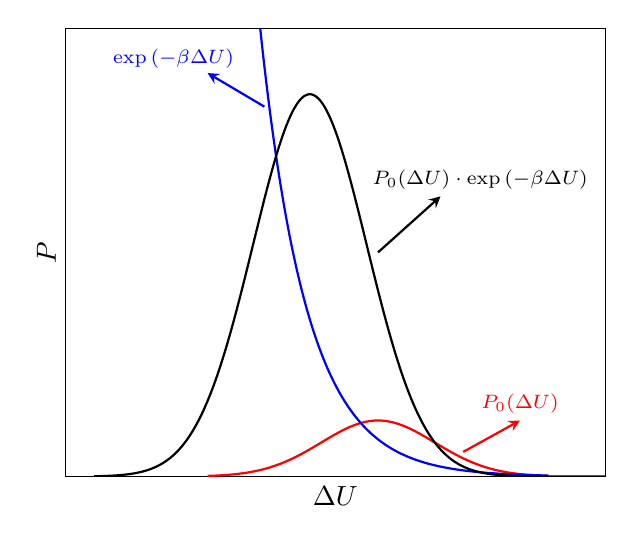
\begin{tikzpicture}
	\def\lims{xmin=-6.5,xmax=3,ymin=0.0,ymax=40}
	\begin{axis}[\lims,
	xtick=\empty, ytick=\empty, minor tick num=0, 
	xlabel=$\Delta U$,
	ylabel={$P$},
	%ytick={0,10,...,40},
	]
	% use TeX as calculator:
	\addplot[thick,color=red,domain=-4:2,samples=500] {5*exp(-(x+1)*(x+1)/2)};
	\addplot[thick,color=blue,samples=500,domain=-4:2] {exp(-1.2*x)};
	\addplot[thick,color=black,samples=500,domain=-6:3] {exp(-1.2*x)*5*exp(-(x+1)*(x+1)/2)};
	\draw[thick,red,->,>=stealth] (axis cs:0.5,2.2) to (axis cs:1.5,5.0);
	\draw[thick,blue,->,>=stealth] (axis cs:-3,33) to (axis cs:-4,36);
	\draw[thick,black,->,>=stealth] (axis cs:-1,20) to (axis cs:0.1,25);
	\draw[red] (axis cs:1.5,6.5) node{\scriptsize$P_0(\Delta U)$};
	\draw[blue] (axis cs:-4.6,37.3) node{\scriptsize$\exp{(-\beta \Delta U)}$};
	\draw[black] (axis cs:0.8,26.5) node{\scriptsize$P_0(\Delta U)\cdot \exp{(-\beta \Delta U)}$};
	\end{axis}
	\end{tikzpicture}
	\caption{$P_{0}(\Delta U)$, the Boltzmann factor $\exp(-\beta \Delta U)$ and their product, which is the integrand in Eq.~\ref{Eq:FEM:TP:deltaA7}. The low-$\Delta U$ tail of the integrand is poorly sampled with $P_{0}(\Delta U)$ and, therefore, is known with low statistical accuracy. However, it provides an important contribution to the integral.}\label{Fig:TP:Pdistribution}
\end{figure}

%\begin{figure}[htbp]
%	\centering
%	\includegraphics[width=0.6\textwidth]{figures/TP.pdf}\\
%\caption{$P_{0}(\Delta U)$, the Boltzmann factor $\exp(-\beta \Delta U)$ and their product, which is the integrand in \ref{Eq:FEM:TP:deltaA7}. The low-$\Delta U$ tail of the integrand is poorly sampled with $P_{0}(\Delta U)$ and, therefore, is known with low statistical accuracy. However, it provides an important contribution to the integral.}\label{Fig:TP:Pdistribution}
%\end{figure}
Even though $P_{0}(\Delta U)$ is only rarely an exact Gaussian, it is instructive to consider this case in more detail. If we substitute
\begin{equation}
  P_{0}(\Delta U) = \frac{1}{\sqrt{2\pi}\sigma}\exp{\left[-\frac{(\Delta U - \left \langle \Delta U \right \rangle_{0})^2}{2\sigma^2}\right]}
  \label{Eq:FEM:TP:gaussian}
\end{equation}
where
\begin{equation}
  \sigma^2 = \left \langle \Delta U^2 \right \rangle_{0} - \left \langle \Delta U \right \rangle_{0}^2
  \label{Eq:FEM:TP:variance}
\end{equation}
to Eq.~\ref{Eq:FEM:TP:deltaA7}, we obtain
\begin{equation}
  \exp(-\beta \Delta A) = \frac{C}{\sqrt{2\pi}\sigma} \int \exp{\left[-\frac{\left[\Delta U - \left(\left \langle \Delta U \right \rangle_{0} - \beta \sigma ^2\right)\right]^2}{2\sigma^2}\right]} \diff\Delta U
  \label{Eq:FEM:TP:expdeltaA}
\end{equation}
Here,
\begin{equation}
  C = \exp{\left[-\beta \left(\left \langle \Delta U \right \rangle_{0} - \frac{1}{2} \beta \sigma ^2\right)\right]}
  \label{Eq:FEM:TP:C}
\end{equation}
is independent of $\Delta U$. It can be seen from Eq.~\ref{Eq:FEM:TP:expdeltaA} that from $P_{0}(\Delta U)$ to $\exp{(-\beta \Delta U)}P_{0}(\Delta U)$, the maximum shifts to the left by $\beta \sigma ^2$, which is proportional to the variance of the Gaussian distribution $P_{0}(\Delta U)$, $\sigma^2$. In other words, the wider the distribution $P_{0}(\Delta U)$, the slower the convergence of TP calculation is. For the number of samples required to ensure the convergence of the TP calculation, the readers may refer to Ref.~\cite{GorePNAS2003}.

If $P_{0}(\Delta U)$ is Gaussian, the integral in Eq.~\ref{Eq:FEM:TP:expdeltaA} can be evaluated analytically using cumulant expansion (see appendix~\ref{chapter:Appendix:CE})
\begin{equation}
  \Delta A = \left< \Delta U \right>_{0} - \frac{1}{2} \beta \sigma ^2.
  \label{Eq:FEM:TP:deltaA8}
\end{equation}
If the distribution of $\Delta U$ deviates from Gaussian, there will be extra terms measuring the skewness of Gaussian. With the leading term, $\Delta A$ becomes
\begin{equation}
  \Delta A = \left< \Delta U \right>_{0} - \frac{1}{2} \beta \sigma ^2 + \frac{\beta^2}{6} \left(\left<\Delta U^3\right>_0-3\left<\Delta U^2\right>_0\left<\Delta U\right>_0+2\left<\Delta U\right>_0^3\right).
  \label{Eq:FEM:TP:deltaA9}
\end{equation}
%The overlap matrix\cite{KlimovichJCAMD2015} is a useful metric in characterizing the magnitude of overlap in the phase space. It is recommended to be used as a consistency check, as in the case of the TP-based methods. If the weight of each of the $N$ samples $x_{n}$ (collected from all $K$ states) in the $i$th state as:
%\begin{equation}
%W_{n,i}(x_{n}) = \frac{e^{\beta G_{i} - \beta U_{i}(x_{n})}}{\sum_{k=1}^{K} N_{k}e^{\beta G_{k}-\beta U_{k}(x_{n})}}
%\label{Eq:FEM:TP:weights}
%\end{equation}
%Then, the overlap matrix is a $K \times K$ matrix with entries:
%\begin{equation}
%O_{i,j} = \sum_{n=1}^{N}\frac{N_{i} e^{\beta G_{i} - \beta U_{i}(x_{n})}}{\sum_{k=1}^{K} N_{k}e^{\beta G_{k}-\beta U_{k}(x_{n})}}\frac{e^{\beta G_{j} - \beta U_{j}(x_{n})}}{\sum_{l=1}^{L} N_{l}e^{\beta G_{l}-\beta U_{l}(x_{n})}}
%\label{Eq:FEM:TP:om}
%\end{equation}

In 2002, Jarzynski proposed a generalized free energy perturbation method termed ``targeted free energy perturbation''.\cite{JarzynskiPRE2002} This method generalizes the free energy perturbation method between two states, $A$ and $B$, by introducing an intermediate state $A^\prime(\mathbf{y})$ by mapping $\mathcal{M}$ from the microstate of the system $\mathbf{x}$ to another one $\mathbf{y}$ in the configuration space or phase space
\begin{equation}
	\mathcal{M}: \mathbf{x} \to \mathbf{y}(\mathbf{x}),
\end{equation}
The potential energy function of the mapped state $A^\prime(\mathbf{y})$ is
\begin{equation}
	U_{A^\prime}(\mathbf{y})=U_A(\mathbf{x})+\beta^{-1}\ln J(\mathbf{x}),
\end{equation}
where $J(\mathbf{x})=|\partial \mathbf{y}/\partial \mathbf{x}|$ is the Jacobian of the mapping $\mathcal{M}$. Zhu et al also used this transformation, but for enhancing conformational sampling.\cite{ZhuPRL2002} The Helmholtz free energy difference between state $A$ and state $A^\prime$ is zero by noticing that
\begin{align*}
	\Delta F_{A^\prime A}=&-\beta^{-1}\ln\frac{Z_{A^\prime}}{Z_A}\notag\\
	                     =&-\beta^{-1}\ln \frac{\displaystyle\int e^{-\beta U_{A^\prime}(\mathbf{y})}\diff y}{Z_A}\notag\\
	                     =&-\beta^{-1}\ln \frac{\displaystyle\int e^{-\beta (U_{A^\prime}(\mathbf{y})-U_A(\mathbf{x}))}e^{-\beta U_A(\mathbf{x})}\diff y}{Z_A}\notag\\
	                     =&-\beta^{-1}\ln \frac{\displaystyle\int J^{-1}(\mathbf{x})e^{-\beta U_A(\mathbf{x})}\diff y}{Z_A}\notag\\
	                     =&-\beta^{-1}\ln \frac{\displaystyle\int e^{-\beta U_A(\mathbf{x})}\diff x}{Z_A}\notag\\
	                     =&0.
\end{align*}
The calculation of the free energy difference between state $A$ and state $B$ can be replaced by the calculation of free energy difference between state $A^\prime$ and state $B$. The latter can be written as
\begin{align}
	\Delta F_{BA^\prime}=&-\beta^{-1}\ln {\int e^{-\beta (U_B(\mathbf{y})-U_{A^\prime}(\mathbf{y}))}\rho_{A^\prime}(\mathbf{y})\diff \mathbf{y}}\notag\\
	                    =&-\beta^{-1}\ln {\int e^{-\beta \Phi(\mathbf{x})}\rho_{A}(\mathbf{x})\diff \mathbf{x}}
\end{align}
in which 
\begin{align}
	\Phi(\mathbf{x})\equiv& U_B(\mathbf{y}) - U_{A^\prime}(\mathbf{y})\notag\\
	                =&U_B(\mathbf{y})-U_A(\mathbf{x})-\beta^{-1}\ln J(\mathbf{x}),
\end{align}
and the relationship between the distributions
\begin{equation}
	\rho_{A^\prime}(\mathbf{y})=\rho_{A}(\mathbf{x})/J(\mathbf{x})
	\label{Eq:FEM:TP:TFEPdistribution}
\end{equation}
has been invoked.

As a special case $\mathcal{M}: \mathbf{x} \to\mathbf{x}$,
\begin{equation}
	\Phi(\mathbf{x})\equiv U_B(\mathbf{x})-U_A(\mathbf{x}),
\end{equation}
and it reduces to the traditional free energy perturbation. It implies that there may exist an invertible mapping $\mathcal{M}$ for which the average of $\exp\{-\beta \Phi\}$ converges more rapidly than the average of $\exp\{-\beta (U_B-U_A)\}$. It can also be asserted that
\begin{align}
	e^{-\beta \Delta F}=&\left<e^{-\beta \Phi}\right>_A\notag\\
	                =&\int \diff \mathbf{x}\, \rho(\mathbf{x})e^{-\beta \Phi(\mathbf{x})}\notag\\
	                =&\int \diff\phi \int \diff \mathbf{x}\, \rho(\mathbf{x})e^{-\beta \Phi(\mathbf{x})}\delta(\Phi(\mathbf{x})-\phi)\notag\\
	                =&\int \diff\phi\, e^{-\beta \phi}\int \rho(\mathbf{x})\delta(\Phi(\mathbf{x})-\phi)\diff \mathbf{x}\notag\\
	                =&\int \diff\phi\, e^{-\beta \phi} p(\phi|\mathcal{M}),
\end{align}
where $p(\phi|\mathcal{M})$ is the distribution of values of $\phi=\Phi(\mathbf{x})$ for $\mathbf{x}$ sampled from $A$. In practice, $\Delta F$ can be estimated by averaging $\exp{(-\beta \Phi)}$ over a finite number of sampled microstates $\mathbf{x}_1,\,\mathbf{x}_2,\dots,\mathbf{x}_N$
\begin{equation}
	\Delta F=-\beta^{-1}\ln\frac{1}{N}\sum_{n=1}^N e^{-\beta \Phi(\mathbf{x}_n)}.
\end{equation}
The rate of convergence depends on the choice of $\mathcal{M}$. A perfect mapping $\mathcal{M}^\ast$ that transforms $A$ exactly onto $B$, we will find from Eq.~\ref{Eq:FEM:TP:TFEPdistribution} that
\begin{equation}
	\frac{1}{Z_B}e^{-\beta E_B(\mathbf{y})}=\frac{1}{Z_A}e^{-\beta E_A(\mathbf{x})}/J(\mathbf{x}),
\end{equation}
which leads to
\begin{equation}
	p(\phi|\mathcal{M}^\ast)=\delta (\phi-\Delta F).
\end{equation}
Then the convergence of the finite sampling is immediate: $\Phi(\mathbf{x})=\Delta F$ for every sampled $\mathbf{x}$. Although constructing a perfect transformation is usually impossible for real-world problems, a transformation that keeps a narrow distribution of $\phi$'s, which implies good overlap between the transformed state and state $B$, can accelerate the convergence of the generalized free energy perturbation calculations.

In 2009, Hahn and Then extended this idea and proposed a bidirectional formulation as a generalized Bennett Acceptance Ratio method\cite{HahnPRE2009}.
They began with the identity
\begin{equation}
	\frac{\rho_{A^\prime}(\mathbf{y}(\mathbf{x}))}{\rho_B(\mathbf{y}(\mathbf{x}))}=e^{\beta\left[\Phi(\mathbf{x})-\Delta F\right]}\qquad \forall \mathbf{x}\in \Gamma_0.
\end{equation}
Multiplying both sides with $\delta [W-\Phi(\mathbf{x})]\rho_B(\mathbf{y}(\mathbf{x}))$ and integrating with respect to $\mathbf{y}$, the left-hand side yields
\begin{align}
	\int_{\mathbf{y}(\Gamma_A)}&\delta[W-\Phi(\mathbf{x})]\rho_{A^\prime}(\mathbf{y}(\mathbf{x}))\diff \mathbf{y}\notag\\
	                          =&\int_{\Gamma_0}\delta[W-\Phi(\mathbf{x})]\rho_A(\mathbf{x})\diff \mathbf{x}\notag\\
	                          =&p(W|A;\mathcal{M}),
\end{align}
and the right-hand side yields
\begin{align}
	\int_{\mathbf{y}(\Gamma_A)}&e^{\beta\left[\Phi(\mathbf{x})-\Delta F\right]}\delta[W-\Phi(\mathbf{x})]\rho_B(\mathbf{y})\diff \mathbf{y}\notag\\
	                          =&e^{\beta\left[W-\Delta F\right]}\int_{\mathbf{y}(\Gamma_A)}\delta[W-\Phi(\mathbf{x})]\rho_B(\mathbf{y})\diff \mathbf{y}\notag\\
	                          =&e^{\beta\left[W-\Delta F\right]}p(W|B;\mathcal{M}),
\end{align}
where $p(W|A;\mathcal{M})$ ($p(W|B;\mathcal{M})$) is the probability density for the outcome of a specific value of the generalized work $W$ in forward (reverse) direction subject to the map $\mathcal{M}$ when sampled from $\rho_A$ ($\rho_B$). Therefore,
\begin{equation}
	\frac{p(W|A;\mathcal{M})}{p(W|B;\mathcal{M})}=e^{\beta\left[W-\Delta F\right]}.
	\label{Eq:FEM:TP:FluctTheo}
\end{equation}
Bayes theorem,
\begin{equation}
	p(W|Y)p_Y=p(Y|W)p(W), \quad \text{with $Y=A$ or $B$}
	\label{Eq:FEM:TP:Bayes}
\end{equation}
implies the ``balance'' equation
\begin{align}
	p_B\int p(A|W)p(W|B)\diff W=&\int p(A|W)p(B|W)p(W)\diff W\notag\\
	                           =&\int p(B|W)p(W|A)p_A\diff W\notag\\
	                           =&p_A\int p(B|W)p(W|A)\diff W,
	                           \label{Eq:FEM:TP:BalEq}
\end{align}
or $p_B\left<p(A|W)\right>_B=p_A\left<p(B|W)\right>_A$.

Combining Eq.~\ref{Eq:FEM:TP:FluctTheo} and Eq.~\ref{Eq:FEM:TP:Bayes} leads to
\begin{equation}
	\frac{p(A|W)}{p(B|W)}=e^{\beta(W-C)}
\end{equation}
with
\begin{equation}
	C=\Delta F+\frac{1}{\beta}\ln{\frac{p_B}{p_A}}.
\end{equation}
With the normalization condition $p(A|W)+p(B|W)=1$, it yields
\begin{equation}
	p(A|W)=\frac{1}{1+e^{\beta(C-W)}}
\end{equation}
and
\begin{equation}
	p(B|W)=\frac{e^{\beta(C-W)}}{1+e^{\beta(C-W)}}=\frac{1}{1+e^{\beta(-C+W)}}.
\end{equation}
Replacing both, the ensemble averages by sample averages and the ratio $\frac{p_B}{p_A}$ by $\frac{n_B}{n_A}$, the balance equation results in
\begin{equation}
	\sum_{j=1}^{n_B}\frac{1}{1+\frac{n_B}{n_A}\exp{\left(\beta\widehat{\Delta F}_{AB}-\beta W^j_B\right)}}=	\sum_{i=1}^{n_A}\frac{1}{1+\frac{n_B}{n_A}\exp{\left(-\beta\widehat{\Delta F}_{AB}+\beta W^i_A\right)}}.
\end{equation}
They also suggested using Kullback-Leibler divergence to characterize the similarity between the mapped state $A^\prime$ and state $B$.

Ding and Zhang further extended this idea and integrated BAR with deep generative model and developed an efficient free energy method DeepBAR.\cite{DingJPCL2021}
\clearpage 
\subsection{Thermodynamic Integration\label{Sec:FEM:TI}}
Thermodynamic Integration (TI) method was proposed by Kirkwood.\cite{KirkwoodJCP1935}. If the free energy, $A$, is a continuous function of $\lambda$, the free energy difference between two states corresponding to $\lambda=0$ and $\lambda=1$ can be computed via
\begin{equation}
\Delta A = \int_{0}^{1} \frac{\partial{A(\lambda)}}{\partial{\lambda}} \diff\lambda.
\label{Eq:FEM:TI:deltaA1TI}
\end{equation} 
With
\begin{equation}
A(\lambda) = -\beta^{-1}\ln Q(\lambda),
\label{Eq:FEM:TI:Alambda}
\end{equation} 
the partial derivative can be expressed as
\begin{align}
\frac{\partial{A(\lambda)}}{\partial{\lambda}} =& -\beta^{-1} \left[ \frac{\partial{\ln{Q(\lambda)}}}{\partial{\lambda}} \right] \notag\\
=&-\frac{\beta^{-1}}{Q(\lambda)}\frac{\partial{Q(\lambda)}}{\partial{\lambda}}.
\label{Eq:FEM:TI:deltaA2TI}
\end{align} 
From the definition of $Q$
\begin{equation}
Q_{NVT}(\lambda) = \frac{1}{{h}^{3N}N!} \iint \exp[-\beta H(\mathbf{x},\mathbf{p}_{x},\lambda)] \diff\mathbf{x}\diff\mathbf{p}_\mathbf{x},
\label{Eq:FEM:TI:PFTI}
\end{equation}
we have
\begin{align}
\frac{\partial{Q(\lambda)}}{\partial{\lambda}} =&\frac{1}{{h}^{3N}N!} \iint \frac{\partial}{\partial{\lambda}}\exp[-\beta H(\mathbf{x},\mathbf{p}_{x},\lambda)] \diff\mathbf{x}\diff\mathbf{p}_\mathbf{x}\notag\\
=& -\frac{\beta}{{h}^{3N}N!} \iint \frac{\partial{H(\mathbf{x},\mathbf{p}_{x},\lambda)}}{\partial{\lambda}}\exp[-\beta H(\mathbf{x},\mathbf{p}_{x},\lambda)] \diff\mathbf{x}\diff\mathbf{p}_\mathbf{x}.
\label{Eq:FEM:TI:PPF2}
\end{align}
Substituting back into the expression for $\partial{A}/\partial{\lambda}$ yields
\begin{align}
\frac{\partial{A(\lambda)}}{\partial{\lambda}} =& \frac{1}{{h}^{3N}N!}\frac{1}{Q(\lambda)} \iint \frac{\partial{H(\mathbf{x},\mathbf{p}_{x},\lambda)}}{\partial{\lambda}}\exp[-\beta H(\mathbf{x},\mathbf{p}_{x},\lambda)] \diff\mathbf{x}\diff\mathbf{p}_\mathbf{x}, \notag\\
=& \frac{1}{{h}^{3N}N!}\iint \frac{\partial{H(\mathbf{x},\mathbf{p}_{x},\lambda)}}{\partial{\lambda}}\cdot\frac{\exp[-\beta H(\mathbf{x},\mathbf{p}_{x},\lambda)]}{Q(\lambda)} \diff\mathbf{x}\diff\mathbf{p}_\mathbf{x},\notag \\
=& \left \langle \frac{\partial{H(\mathbf{x},\mathbf{p}_{x}, \lambda)}}{\partial{\lambda}} \right \rangle_{\lambda}
\label{Eq:FEM:TI:PA2}
\end{align}
Thus, the basic TI formula is
\begin{equation}
\Delta A = \int_{0}^{1}\left \langle \frac{\partial{H(\mathbf{x},\mathbf{p}_{x},\lambda)}}{\partial{\lambda}} \right \rangle_{\lambda} \diff\lambda
\label{Eq:FEM:TI:TI}
\end{equation} 
where $\left \langle \cdots \right \rangle _{\lambda}$ corresponds to the ensemble average obtained using the Hamiltonian $H(\lambda)$. In practice, the ensemble of configurations can be obtained by molecular dynamics or Monte Carlo simulations. It is common practice in free energy calculations to use the coupling parameter $\lambda$ for defining the transformation from the initial state $A$ with Hamiltonian $H_{A}$ to the final state $B$ with Hamiltonian $H_{B}$. The simplest coupling is linear transformation as
\begin{equation}
H(\lambda) = (1-\lambda) H_{A} + \lambda H_{B},
\end{equation}
for which
\begin{equation}
	\frac{\partial{H(\lambda)}}{\partial{\lambda}}=H_B-H_A. 
\end{equation}
However, this simple mixing scheme does not provide the optimal alchemical transformation pathway. Better schemes are possible, for instance the minimum variance path (MVP)\cite{BlondelJCC2004} and the optimal transport pathway\cite{DecherchiJPCL2023}. 
The accuracy of TI integral formula depends on the exactness of the numerical integration method.\cite{PaliwalJCTC2011} Practically, the integrand in Eq.~\ref{Eq:FEM:TI:TI} needs to be evaluated over a number of discrete points $\lambda_{i}$, and then be summed up to give the free energy difference between $\lambda=0$ and $1$, for instance via the trapezoidal rule
\begin{equation}
\Delta A = \sum_{i=0}^{N-1}\frac{1}{2}\left(\left \langle \frac{\partial{H(\lambda)}}{\partial{\lambda}} \right \rangle_{\lambda_{i}} + \left \langle\frac{\partial{H(\lambda)}}{\partial{\lambda}} \right \rangle_{\lambda_{i+1}}\right)
(\lambda_{i+1}-\lambda_i).
\label{Eq:FEM:TI:dTI}
\end{equation} 
A finite number of $\lambda_{i}$ values between 0 and 1 are chosen and for each of them a complete molecular dynamics simulation is carried out resulting in an ensemble of configurations generated with $H(\lambda_{i})$.
The ensemble average of the derivative of the Hamiltonian with respect to $\lambda$ is then calculated for each $\lambda_{i}$.
	
In addition to summation method, the simplest numerical integration is to evaluate the integrand at the midpoint:
\begin{equation}
\Delta A \simeq \left \langle \frac{\partial{H(\lambda)}}{\partial{\lambda}} \right \rangle_{\lambda=\frac{1}{2}}
\label{Eq:FEM:TI:TI1}
\end{equation} 
This might be a good first thing to do to get some impression of what is going on, but is only accurate for very smooth or small changes. %Gaussian quadrature formulas of higher order are generally more useful:
%\begin{equation}
%\Delta A = \sum_{i}^{} w_{i}\left \langle \frac{\partial{H(\lambda)}}{\partial{\lambda}} \right \rangle_{\lambda_{i}}
%\label{Eq:FEM:TI:Gauss}
%\end{equation} 
%Some weights and quadrature points are given in the table~\ref{tab:Gauss}; other formulas are possible, \cite{HummerJCP1996} but the Gaussian one listed here are probably the most useful. The formulas are always symmetrical about $\lambda = 0.5$, so that $\lambda$ and $(1-\lambda)$ both have the same weight.
	
%\clearpage
%\begin{table*}
%	\caption{\label{tab:Gauss}Abscissas and weights for Gaussian integration.}
%	\newcommand{\rb}[1]{\raisebox{1.5ex}[0t]{#1}}
%	\begin{tabular}{lcccccccccccccccccc}
%		\hline
%	   n&$\lambda_{i}$&$1-\lambda_{i}$&$w_{i}$ \\
%		\hline
%	   1&     0.5&        & 1.0 \\
%		\hline
%	   2& 0.21132& 0.78867& 0.5 \\
%		\hline
%	   3&  0.1127& 0.88729& 0.27777 \\
%		&     0.5&        & 0.44444 \\
%		\hline
%	   5& 0.04691& 0.95308& 0.11846 \\
%		& 0.23076& 0.76923& 0.23931 \\
%		&     0.5&        & 0.28444 \\
%		\hline
%	   7& 0.02544& 0.97455& 0.06474 \\
%		& 0.12923& 0.87076& 0.13985 \\
%		& 0.29707& 0.70292& 0.19091 \\
%		&     0.5&        & 0.20897 \\
%		\hline
%	   9& 0.01592& 0.98408& 0.04064 \\
%		& 0.08198& 0.91802& 0.09032 \\
%		& 0.19331& 0.80669& 0.13031 \\
%		& 0.33787& 0.66213& 0.15617 \\
%		&     0.5&        & 0.16512 \\
%		\hline
%	  12& 0.00922& 0.99078& 0.02359 \\ 
%		& 0.04794& 0.95206& 0.05347 \\
%		& 0.11505& 0.88495& 0.08004 \\
%		& 0.20634& 0.79366& 0.10158 \\
%		& 0.31608& 0.68392& 0.11675 \\
%		& 0.43738& 0.56262& 0.12457 \\
%		\hline
%	\end{tabular} 
%\end{table*}
\clearpage
% !TeX spellcheck = en_US
\subsection{Bennett Acceptance Ratio\label{Sec:FEM:BAR}}
\begin{chapquote}{Professor Savas Dimopoulos, Stanford University}
	``The thing that differentiates scientists is purely an artistic ability to discern what is a good idea, what is a beautiful idea, what is worth spending time on, and most importantly, what is a problem that is sufficiently interesting, yet sufficiently difficult, that is hasn't yet been solved, but the time for solving it has come now.''
\end{chapquote}
Bennett acceptance ratio was developed by Bennett in 1976,\cite{BennettJComputPhys1976} and was re-discovered by Crooks\cite{CrooksPRE2000} for Markovian and balanced dynamics and by Shirts et al\cite{ShirtsPRL2003} using maximum likelihood over 20 years later. The Metropolis function is defined as
\begin{equation}
	M(x)=min\{1,\exp{(-x)}\},
\end{equation}
which has the property 
\begin{equation}
	M(x)/M(-x)=\exp{(-x)}.
\end{equation}

If we make a trial move that keeps the same configuration ($q_{1},\cdots,q_{N}$)
but switches the potential function from $U_{0}$ to $U_{1}$ or vice-versa, 
the acceptance probabilities for such a pair of trial moves must satisfy
the detailed balance
\begin{equation}
	M(U_{1}-U_{0})\exp{(-U_{0})}=M(U_{0}-U_{1})\exp{(-U_{1})}.
\end{equation}

Integrating this identity over all of configuration space and multiplying
by the trivial factors $Q_{0}/Q_{0}$ and $Q_{1}/Q_{1}$, one obtains:

\begin{equation}
	Q_{0}\frac{\displaystyle\int M(U_{1}-U_{0})\exp{(-U_{0})}\diff\mathbf{{q}}}{Q_{0}}=Q_{1}\frac{\displaystyle\int M(U_{0}-U_{1})\exp{(-U_{1})}\diff\mathbf{{q}}}{Q_{1}},
\end{equation}
or simply

\begin{equation}
	\frac{Q_{0}}{Q_{1}}=\frac{\langle M(U_{0}-U_{1})\rangle_{1}}{\langle M(U_{1}-U_{0})\rangle_{0}}.\label{eq:FEM:BAR:MetropolisRatio}
\end{equation}

The physical meaning of this formula is that a Monte Carlo calculation
that includes potential-switching trial moves would distribute configurations
between $U_{1}$ and $U_{0}$ in the ratio of their configurational
integrals. 

A formula more general than Eq.~\ref{eq:FEM:BAR:MetropolisRatio} can be written as
\begin{equation}
	\frac{Q_{0}}{Q_{1}}=\frac{Q_{0}}{Q_{1}}\frac{\displaystyle\int W\exp{(-U_{0}-U_{1})}\diff\mathbf{{q}}}{\displaystyle\int W\exp{(-U_{1}-U_{0})}\diff\mathbf{{q}}}=\frac{\langle W\exp{(-U_{0})}\rangle_{1}}{\langle W\exp{(-U_{1})}\rangle_{0}},\label{eq:FEM:BAR:weightedratio}
\end{equation}
where $W$ is an arbitrary weighting function.

Optimization of the free energy estimate is most easily carried out in the limit of large sample sizes. Let the available data consist
of $n_{0}$ statistically independent configurations from the $U_{0}$ ensemble and $n_{1}$ from the $U_{1}$ ensemble, and let the data
be used in Eq.~\ref{eq:FEM:BAR:weightedratio} to obtain a finite-sample estimate of the reduced free energy difference $\Delta A=A_{1}-A_{0}=\ln{(Q_{0}/Q_{1})}$.
Using the error propagation law of uncorrelated variables ($covar(x_1,x_2)=0$),\cite{BerendsenBook2011}
\begin{equation}
	\delta^2\left[y(x_{1},x_{2})\right]=\left(\frac{\partial y}{\partial x_{1}}\right)^{2}\delta^2(x_{1})+\left(\frac{\partial y}{\partial x_{2}}\right)^{2}\delta^2(x_{2}).
\end{equation}

Thus we have the variance of $\Delta A$
\begin{eqnarray}
	\delta^2(\Delta A) & = & \left(\frac{\partial\Delta A}{\partial Q_{0}}\right)^{2}\delta^2Q_0+\left(\frac{\partial\Delta A}{\partial Q_{1}}\right)^{2}\delta^2Q_1\notag\\
	& = & \left(\frac{1}{Q_{0}}\right)^{2}\delta^2Q_0+\left(-\frac{1}{Q_{1}}\right)^{2}\delta^2Q_1\notag\\
	& = & \left(\frac{1}{Q_{0}}\right)^{2}\delta^2Q_0+\left(\frac{1}{Q_{1}}\right)^{2}\delta^2Q_1.
\end{eqnarray}

With the definition of variance $\delta^2X=\left\langle X^{2}\right\rangle -\left\langle X\right\rangle ^{2}$,
we have 
\begin{eqnarray}
	\delta^2Q_0 & = & \delta^2\left\langle W\exp{(-U_{0})}\right\rangle_{1}\notag\\
	& = & \delta^2\left(\frac{1}{n_1}\sum_{i=1}^{n_1}W_{i}\exp{\left(-U_{0}(i)\right)}\right)\notag\\
	& = & \sum_{i=1}^{n_{1}}\left(\frac{1}{n_{1}}\right)^{2}\delta^2\left(W_{i}\exp{\left(-U_{0}(i)\right)}\right)\notag\\
	& = & \frac{1}{n_{1}}\delta^2\left(W_{i}\exp{\left(-U_{0}(i)\right)}\right)\notag\\
	& = & \frac{1}{n_{1}}\left\{ \left< \left[W\exp{(-U_{0})}\right]^{2}\right>_{1}-\left[\left< W\exp{(-U_{0})}\right>_{1}\right]^{2}\right\}\notag\\
	& = & \frac{1}{n_{1}}\left\{ \left< W^{2}\exp{(-2U_{0})}\right>_{1}-\left[\left< W\exp{(-U_{0})}\right>_{1}\right]^{2}\right\},
\end{eqnarray}
which shows that the variance of the mean of the samples equals to the variance of the samples divided by the number of samples.

With sufficiently large sample sizes, the error of this estimate will
be nearly Gaussian, and its expected square is exactly the variance
of $\Delta A$ 
\begin{align}
	\delta^2 & (\Delta A_{est}-\Delta A)\nonumber \\
	\approx & \frac{\langle W^{2}\exp{(-2U_{1})}\rangle_{0}}{n_{0}[\langle W\exp{(-U_{1})}\rangle_{0}]^{2}}+\frac{\langle W^{2}\exp{(-2U_{0})}\rangle_{1}}{n_{1}[\langle W\exp{(-U_{0})}\rangle_{1}]^{2}}-\frac{1}{n_{0}}-\frac{1}{n_{1}}\nonumber \\
	= & \frac{\displaystyle\int\left[\frac{Q_{0}}{n_{0}}\exp{(-U_{1})}+\frac{Q_{1}}{n_{1}}\exp{(-U_{0})}\right]W^{2}\exp{(-U_{0}-U_{1})}\diff\mathbf{q}}{\left[\displaystyle\int W\exp{(-U_{0}-U_{1})}\diff\mathbf{q}\right]^{2}}\notag\\
	  &-\frac{1}{n_{0}}-\frac{1}{n_{1}}.\label{eq:FEM:BAR:expectation}
\end{align}

To minimize it with respect to $W$, we have
\begin{equation}
	W=const\times\left(\frac{Q_{0}}{n_{0}}\exp{(-U_{1})}+\frac{Q_{1}}{n_{1}}\exp{(-U_{0})}\right)^{-1}.
	\label{eq:FEM:BAR:W}
\end{equation}

Substituting this into Eq.~\ref{eq:FEM:BAR:weightedratio} yields
\begin{equation}
	\frac{Q_{0}}{Q_{1}}=\frac{\langle f(U_{0}-U_{1}+C)\rangle_{1}}{\langle f(U_{1}-U_{0}-C)\rangle_{0}}\exp{(+C)},
	\label{Eq:FEM:BAR:BAR}
\end{equation}
where
\begin{equation}
	C=\ln\frac{Q_{0}n_{1}}{Q_{1}n_{0}},
	\label{Eq:FEM:BAR:C}
\end{equation}
and $f$ denotes the Fermi function
\begin{equation}
	f(x)=\frac{1}{1+\exp{(+x)}}.
\end{equation}
It can also be expressed as\cite{ShirtsPRL2003}
\begin{equation}
	n_1\langle f(U_{0}-U_{1}+C)\rangle_{1}=n_0\langle f(U_{1}-U_{0}-C)\rangle_{0}.
\end{equation}
It should be noted that Eq.~\ref{Eq:FEM:BAR:BAR} is true for any $C$, which is actually a shift for one of the potential function. But the particular value specified in Eq.~\ref{Eq:FEM:BAR:C} minimizes the expected square error given the finite numbers ($n_0$ and $n_1$) of samples.

The variance of $\Delta A$ can be obtained by substituting Eq.~\ref{eq:FEM:BAR:W} into Eq.~\ref{eq:FEM:BAR:expectation}, and is 
\begin{align}
	\delta^2 \Delta A =&\frac{\left<f^2(U_{1}-U_{0}-C)\right>_0}{n_0\left<f(U_{1}-U_{0}-C)\right>_0^2}+\frac{\left<f^2(U_{0}-U_{1}+C)\right>_1}{n_1\left<f(U_{0}-U_{1}+C)\right>_1^2}-\frac{1}{n_0}-\frac{1}{n_1}\notag\\
	=&\left(\int \frac{n_0n_1\rho_0\rho_1}{n_0\rho_0+n_1\rho_1}\diff \mathbf{q}\right)^{-1}-\frac{n_0+n_1}{n_0n_1},
\end{align}
in which $\rho_i=\exp{(-U_i)}/Q_i$ is the probability.

It is worth emphasizing that Bennett acceptance ratio is asymptotically unbiased, and no other asymptotically unbiased estimator has lower asymptotic mean-squared error. However, it is not clear whether its behavior is always better than other estimators with finite sample sizes.

Shirts et al showed that BAR can be interpreted in terms of the maximum likelihood estimate of the free energy difference given a set of work values in the forward and reverse directions.\cite{ShirtsPRL2003} Starting from (refer to Appendix~\ref{chapter:Appendix:DeltaUDistributions} for the proof)
\begin{equation}
	\ln\left[\frac{P(W|F)}{P(-W|R)}\right]=\beta (W-\Delta F),
	\label{eq:FEM:BAR:distributionratio}
\end{equation}
where $P(W|F)$ ($P(W|R)$) is probability distribution for the work from the two states in the forward (reverse) direction, which can also be thought as the conditional probability of a work value given that it is a forward (reverse) measurement. To simplify the notation, the work $W$ from the reverse direction will be replaced by $-W$. Using the fact that $P(F|W)+P(R|W)=1$, the ratio can be rewritten as
\begin{equation}
	\frac{P(W|F)}{P(R|R)}=\frac{P(F|W)P(R)}{P(R|W)P(F)}=\frac{P(F|W)}{1-P(F|W)}\frac{P(R)}{P(F)}.
\end{equation}
It can be realized that $P(R)/P(F)=n_R/n_F$, where $n_F$ ($n_R$) is the number of forward (reverse) measurement. Defining $M=\ln{n_F/n_R}$, Eq.~\ref{eq:FEM:BAR:distributionratio} can be rewritten as
\begin{equation}
	\ln\frac{P(F|W)}{1-P(F|W)}=(M+W-\Delta F),
\end{equation}
which leads to
\begin{align}
	P(F|W_i)=&\frac{1}{1+\exp[-(M-W_i-\Delta F)]},\\
	P(R|W_i)=&\frac{1}{1+\exp[M-W_i-\Delta F]}
\end{align}
for a single work measurement $W_i$, given a value of the free energy difference $\Delta F$.

Given a value for $\Delta F$, the overall likelihood $L$ becomes
\begin{equation}
	L(\Delta F)=\prod_{i=1}^{n_F}P(F|W_i)\prod_{i=1}^{n_R}P(R|W_i).
\end{equation}
The most likely value of $\Delta F$ is the value that maximizes the (log) likelihood, therefore we have
\begin{align}
	0=\frac{\partial \log L(\Delta F)}{\partial \Delta F}=&-\sum_{i=1}^{n_F}\frac{1}{1+\exp\left[M+W_i-\Delta F\right]}\notag\\
	                                                      &+\sum_{j=1}^{n_R}\frac{1}{1+\exp\left[-(M+W_j-\Delta F)\right]},
\end{align}
which equivalent to the BAR method.
\clearpage 
% !TeX spellcheck = en_US
\subsection{Weighted Histogram Analysis Method\label{Sec:FEM:WHAM}}
The weighted histogram analysis method is a generalization of the histogram method developed by Ferrenberg and Swendsen.\cite{FerrenbergPRL1989}
\subsubsection{Weighted Histogram Analysis Method for Parallel Tempering\label{Sec:FEM:WHAM_REMD}}
The following derivation quite follows Ref.~\cite{ChoderaJCTC2007}.
One of the central quantities in statistical mechanics is configurational integral $Z$, which in textbook is often written as
\begin{equation}
Z=\int \exp{(-\beta U(\mathbf{R}))}\diff\mathbf{R}.
\end{equation}
This is an integral in coordinate space. It also can be written as an integral in energy space
\begin{equation}
Z=\int \Omega(U)\exp{(-\beta U)}\diff U,
\end{equation}
where $\Omega(U)$ is density of states and $\Omega(U)\Delta U$ is the number of states in the region $U-\Delta U/2<U<U+\Delta U/2$. Accordingly, the statistical expectation of an operator $\mathbf{A}$ can be calculated by
\begin{equation}
\langle \mathbf{A}\rangle=\frac {\displaystyle\int \mathbf{A}(U)\Omega(U)\exp{(-\beta U)}\diff U}{\displaystyle\int \Omega(U)\exp{(-\beta U)}\diff U},
\end{equation}
where
\begin{equation}
\mathbf{A}(U^\prime)=\frac{\displaystyle\int \delta (U(\mathbf{R})-U^\prime)\mathbf{A}(\mathbf{R})\diff \mathbf{R}}{\displaystyle\int \delta (U(\mathbf{R})-U^\prime)\diff\mathbf{R}},
\end{equation}
is the average of $\mathbf{A}$ over all the samples with an energy $U^\prime$. Therefore, the core objective is to calculate $\Omega(U)$.

Suppose we have one trajectory with $N$ snapshots denoted as $\{\mathbf{R}_n\}$. We then discretize the energy space into $M$ bins with width $\Delta U$, and count the number of snapshots into each bin. For convenience, we define $\psi_m(U)$ as
\begin{equation}
	\psi_m(U)= 
	\left\{ 
	\begin{array}{rl} 
	1 & \text{if }U\in \left[ U_m-\Delta U/2, U_m+\Delta U/2\right)\\ 
	0 & \text{otherwise}\\  
	\end{array} 
	\right. 
\end{equation}
Then the histogram for the $m$th energy bin is
\begin{equation}
	H_{m}=\sum\limits_{n=1}^{N}\psi_{m}(U(\mathbf{R}_n))=N\cdot \frac 1 N\sum\limits_{n=1}^{N}\psi_{m}(U(\mathbf{R}_n))=N\cdot\left<\psi_m\right>,
\end{equation}
with variances (see Appendix~\ref{chapter:Appendix:Uncertainty})
\begin{align}
	\delta^2 H_m=&N^2\delta^2(\left<\psi_m\right>)\notag\\
	            =&g_m N\left(\left<{\psi_m}^2\right>-\left<\psi_m\right>^2\right)\notag\\
	            =&g_m N\left(\left<\psi_m\right>-\left<\psi_m\right>^2\right)\notag\\
	            =&g_m H_m\left(1-\frac{H_m}{N}\right).
\end{align}

%A sample histogram in 2D space is shown in Fig.~\ref{Fig:FEM:WHAM:histogram}.
%\begin{figure}[htbp]
%	\centering
%    \begin{tikzpicture}
%        \begin{axis}[xtick=\empty, ytick=\empty, ztick=\empty, minor tick num=0,view/h=40]
%        
%          \addplot3[surf,
%          mesh/color input=colormap,
%          colormap/hot,
%          domain=-180:180, y domain=-180:180,
%          point meta={sin(x)*sin(y)},
%          point meta rel=per plot,
%          point meta min=-1.0, point meta max=1.0,
%          shader=faceted,
%          update limits=false,
%          on layer=axis background,
%          samples=30
%          ] {-1.2};
%          \addplot3[surf, shader=faceted, domain=-180:180, y domain=-180:180, samples=30] 
%          {sin(x)*sin(y)};
%%         \addplot3[surf, shader=faceted, domain=-180:180, y domain=-180:180, samples=20, color=black, point meta rel=per plot, point meta={sin(x)*sin(y)} ] {-1.0};
%
%        \end{axis}
%    \end{tikzpicture}
%    \caption{A sample histogram in 2D space, for instance potential energy and a reaction coordinate $\xi$.}\label{Fig:FEM:WHAM:histogram}
%\end{figure}
A sample histogram is shown in Fig.~\ref{Fig:FEM:WHAM:histogram}.
\begin{figure}[htbp]
	\centering
	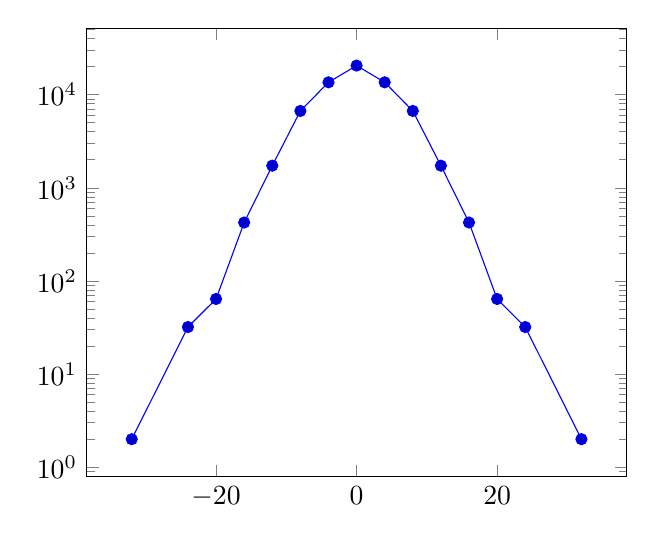
\begin{tikzpicture}
		\begin{axis}[ymode=log,]
	    	\addplot plot coordinates{
		    	(-32.0, 2)
			    (-24.0, 32)
			    (-20.0, 64)
			    (-16.0, 424)
			    (-12.0, 1728)
			    (-8.0, 6688)
			    (-4.0, 13568)
			    (0.0, 20524)
			    (4.0, 13568)
			    (8.0, 6688)
			    (12.0, 1728)
			    (16.0, 424)
			    (20.0, 64)
			    (24.0, 32)
			    (32.0, 2)
		};
	\end{axis}
	\end{tikzpicture}
	\caption{Density of states of a 4$\times$4 periodic Ising model}\label{Fig:FEM:WHAM:histogram}
\end{figure}

The ratio of the histogram $H_m$ to the total number of snapshots $N$ divided by the bin width $\Delta U$ can be approximately taken as the probability of states in this bin, i.e.,
\begin{equation}
	\frac{\Omega_m\exp{(-\beta U_m)}}{Z}\approx\frac{H_m}{N\Delta U}.
\end{equation}
Therefore,
\begin{align}
	\Omega_m=&\frac{1}{\Delta U}\cdot\frac{H_m}{N}\cdot\frac{Z(\beta)}{\exp{(-\beta U_m)}}\notag\\
	        =&\frac{H_m}{N\Delta U\exp{\left[f-\beta U_m\right]}},
	\label{Eq:FEM:WHAM:DoSsingle}
\end{align}
and variances
\begin{equation}
	\delta^2\Omega_m=\frac{\delta^2 H_m}{\left(N\Delta U\exp{\left[f-\beta U_m\right]}\right)^2},
\end{equation}
in which we have defined a dimensionless free energy $f=-\ln{Z(\beta)}$.

Practically, we may run multiple ($K$) trajectories using, for example, replica exchange molecular dynamics simulations. For each trajectory (index $k$), we have unique estimators for the histogram $H_{mk}$, the density of states $\Omega_{mk}$ and their variances $\delta^2 H_{mk}$ and $\delta^2\Omega_{mk}$ being
\begin{equation}
	H_{mk}=\sum\limits_{n=1}^{N_k}\psi_{m}(U(\mathbf{R}_{kn})),
\end{equation}
\begin{equation}
	\delta^2 H_{mk}=g_{mk}H_{mk}\left(1-\frac{H_{mk}}{N_k}\right),
\end{equation}
\begin{align}
	\Omega_{mk}=\frac{H_{mk}}{N_k\Delta U\exp{\left[f_k-\beta_kU_{m}\right]}},
	\label{Eq:FEM:WHAM:Omega_mk}
\end{align}
and
\begin{equation}
	\delta^2\Omega_{mk}=\frac{\delta^2 H_{mk}}{\left(N_k\Delta U\exp{\left[f_k-\beta_kU_{m}\right]}\right)^2},
\end{equation}
The optimum estimator of the density of states from all the simulations is
\begin{equation}
	\Omega_m=\frac{\sum\limits_{k=1}^K\left[\delta^2\Omega_{mk}\right]^{-1}\Omega_{mk}}{\sum\limits_{k=1}^K\left[\delta^2\Omega_{mk}\right]^{-1}},
	\label{Eq:FEM:WHAM:optimumOmega}
\end{equation}
which is the weighted average of density of states of all the trajectories with the weight reversely proportional to the variances (see Appendix~\ref{chapter:Appendix:Mean}).

To make the expression simpler, here we take some approximations. First, normally the energy space is split into a large number of bins. The histogram in each bin is much smaller than the total number of snapshots, i.e. $H_{mk}\ll N_k$. With this approximation, we have
\begin{align}
	\delta^2 H_{mk}\approx g_{mk}H_{mk}.
\end{align}
The expectation of $H_{mk}$ can be related to the optimum estimator of the density of states, i.e.
\begin{equation}
	\overline{H_{mk}}=N_k\Delta U\Omega_m\exp{(f_k-\beta_kU_m)}.
\end{equation}
Then we have
\begin{equation}
    \delta^2H_{mk}=g_{mk}N_k\Delta U\Omega_m\exp{(f_k-\beta_kU_m)}
    \label{EQ:FEM:WHAM:delta2H_mk}
\end{equation}
and
\begin{equation}
\delta^2\Omega_{mk}=\frac{\Omega_m}{{g_{mk}}^{-1}N_k\Delta U\exp{(f_k-\beta_kU_m)}}.
\label{Eq:FEM:WHAM:delta2Omega_mk}
\end{equation}

Taking Eq.~\ref{Eq:FEM:WHAM:Omega_mk} and Eq.~\ref{Eq:FEM:WHAM:delta2Omega_mk} into Eq.~\ref{Eq:FEM:WHAM:optimumOmega}, we find
\begin{equation}
\Omega_m=\frac{\sum\limits_{k=1}^{K}{g_{mk}}^{-1}H_{mk}}{\sum\limits_{k=1}^{K}{g_{mk}}^{-1}N_k\Delta U\exp{(f_k-\beta_kU_m)}},
\label{Eq:FEM:WHAM:Omega_iteration}
\end{equation}
in which
\begin{equation}
f_k=-\ln \int \Omega(U)\exp{(-\beta_k U)}\diff U=-\ln\sum\limits_{m=1}^M\Omega_m\Delta U\exp{(-\beta_kU_m)}.
\label{Eq:FEM:WHAM:f_k_iteration}
\end{equation}
Obviously, Eq.~\ref{Eq:FEM:WHAM:Omega_iteration} and Eq.~\ref{Eq:FEM:WHAM:f_k_iteration} must be solved iteratively.
Applying the error propagation rule to Eq.~\ref{Eq:FEM:WHAM:Omega_iteration} and using Eq.~\ref{EQ:FEM:WHAM:delta2H_mk}, the variance of $\Omega_m$ is given by
\begin{equation}
\delta^2 \Omega_m=\frac{\Omega_m}{\sum\limits_{k=1}^K{g_{mk}}^{-1}N_k\Delta U\exp{(f_k-\beta_kU_m)}}.
\end{equation}
%and the relative variance is given by
%\begin{equation}
%\frac{\delta^2\Omega_m}{\Omega_m^2}=\left[\sum\limits_{k=1}^K{g_{mk}}^{-1}H_{mk}\right]^{-1}.
%\end{equation}
Using the density of states and its variance, we can estimate the expectation of any configuration function $A(\mathbf{R})$ at any inverse temperature $\beta$
\begin{equation}
\left<A\right>_\beta\approx\frac{\sum\limits_{m=1}^M\Omega_m\Delta U\exp{(-\beta U_m)}A_m}{\sum\limits_{m=1}^M\Omega_m\Delta U\exp{(-\beta U_m)}},
\label{Eq:FEM:WHAM:A}
\end{equation}
where
\begin{equation}
A_m=\frac{\displaystyle\int \diff\mathbf{R}\,A(\mathbf{R})\psi_m(U(\mathbf{R}))}{\displaystyle\int \diff\mathbf{R}\,\psi_m(U(\mathbf{R}))}.
\end{equation}
Using histograms of bin $m$ from all the simulations and defining $H_m=\sum\limits_{k=1}^KH_{mk}$, an estimator of $A_m$ denoted as $\hat{A}_m$ can be calculated as
\begin{equation}
   \hat{A}_m={H_{m}}^{-1}\sum\limits_{k=1}^K\sum\limits_{n=1}^{N_k}\psi_m(U(\mathbf{R}_{kn}))A(\mathbf{R}_{kn}).
   \label{Eq:FEM:WHAM:A_m}
\end{equation}
Taking Eq.~\ref{Eq:FEM:WHAM:A_m} into Eq.~\ref{Eq:FEM:WHAM:A}, we obtain an estimator of $\hat{A}(\beta)$
\begin{align}
\hat{A}(\beta)=&\frac{\sum\limits_{m=1}^M\Omega_m\Delta U\exp{(-\beta U_m)}{H_{m}}^{-1}\sum\limits_{k=1}^K\sum\limits_{n=1}^{N_k}\psi_m(U(\mathbf{R}_{kn}))A(\mathbf{R}_{kn})}{\sum\limits_{m=1}^M\Omega_m\Delta U\exp{(-\beta U_m)}}\\
              =&\frac{\sum\limits_{m=1}^M\Omega_m\Delta U\exp{(-\beta U_m)}{H_{m}}^{-1}\sum\limits_{k=1}^K\sum\limits_{n=1}^{N_k}\psi_m(U(\mathbf{R}_{kn}))A(\mathbf{R}_{kn})}{\sum\limits_{m=1}^M\Omega_m\Delta U\exp{(-\beta U_m)}{H_{m}}^{-1}\sum\limits_{k=1}^K\sum\limits_{n=1}^{N_k}\psi_m(U(\mathbf{R}_{kn}))}\\
              =&\frac{\sum\limits_{k=1}^K\sum\limits_{n=1}^{N_k}w_{kn}(\beta)A_{kn}}{\sum\limits_{k=1}^K\sum\limits_{n=1}^{N_k}w_{kn}(\beta)},
\end{align}
where the per-configuration weights $w_{kn}(\beta)$ is given by
\begin{equation}
w_{kn}(\beta)=\sum\limits_{m=1}^M{H_{m}}^{-1}\psi_m(U(\mathbf{R}_{kn}))\Omega_m\exp{(-\beta U_m)}
\end{equation}

\subsubsection{Weighted Histogram Analysis Method From Minimizing Statistical Error}
In this section, the ``traditional'' derivation method of WHAM are briefly reviewed.\cite{SouailleCPC2001} In the WHAM, the goal is to get an optimal unbiased probability distribution $\rho_{0}(\eta)$, where $\eta$ is a series of discretized histogram bins indexed by $j=1,2,3,...,M$ along a certain reaction coordinate. WHAM can be used to analyze the Umbrella Sampling (US) simulations, where a set of simulations indexed by $i$ or $k=1,2,3,...,S$ are performed with a series of biasing potentials added on the reaction coordinate $\eta$. To consider a reference molecular system with the potential energy $U_{0}(\textbf{x})$, where $\textbf{x}$ is the set of atomic coordinates. The reaction coordinate $\eta$ is a function of the atomic coordinates, i.e. $\eta(\textbf{x})$. To suppose that the $i$th molecular simulation has been performed using potential energy function
\begin{equation}
U_{i}^{(b)}(\eta) = U_{0}(\textbf{x}) + W_{i}(\eta(\textbf{x})),
\label{Eq:FEM:WHAM:biasmd}
\end{equation}
where $W_{i}(\eta(\textbf{x}))$ is the biasing potential added on the reaction coordinate $\eta$, e.g. $W_{i}(\eta)=\frac{1}{2}k_{i}(\eta-\eta_{i})^2$ in a harmonic form. From these simulations a set of normalized biased probability distributions ${\rho_{i}^{(b)}(\eta)}$ can be obtained.
\begin{equation}
\rho_{i}^{(b)}(\eta) = \frac{e^{-\beta U_{i}^{(b)}(\eta)}}{Q_{i}^{(b)}},
\label{Eq:FEM:WHAM:bias}
\end{equation}
where $Q_{i}^{(b)}=\displaystyle\int e^{-\beta U_{i}^{(b)}(\eta)} \diff\eta = e^{-\beta f_{i}^{(b)}}$ and $f_{i}^{(b)}$ is the biased free energy.
The corresponding unnormalized unbiased probability distribution $\rho_{i}^{(u)}(\eta)$ from the $i$th simulation is defined as, 
\begin{align}
\rho_{i}^{(u)}(\eta) = e^{\beta[W_{i}(\eta)-f_{i}^{(b)}]}\rho_{i}^{(b)}(\eta)
\label{Eq:FEM:WHAM:unbias}
\end{align}
In the following, the free energy $f_{i}^{(b)}$ is assumed to be known. 
It has been shown that in the WHAM method, the total normalized unbiased probability distribution $\rho_{0}(\eta)$ can be obtained by a linear $\eta$-dependent combination of the unbiased histograms $\rho_{i}^{(u)}(\eta)$ 
\begin{equation}
\rho_{0}(\eta)=C\sum_{i=1}^{S}p_{i}(\eta)\rho_{i}^{(u)}(\eta),
\label{Eq:FEM:WHAM:unbias0}
\end{equation}  
where $C$ is the normalization factor. $p_i$ is the weight to be optimized, which is under a constraint that
\begin{equation}
\sum_{i=1}^{S}p_{i}(\eta)=1.
\label{Eq:FEM:WHAM:p1}
\end{equation}
These weights are chosen so as to minimize the statistical error made on the total unbiased probability distribution $\rho_{0}(\eta)$, that is, for any given value of $\eta$,
\begin{equation}
\frac{\partial(\sigma^2[\rho_{0}(\eta)])}{\partial p_{i}(\eta)}=0.
\label{Eq:FEM:WHAM:partialp}
\end{equation} 
It can be easily found that $\rho_{0}(\eta)$ satisfies
\begin{align}
\rho_{0}(\eta) = & C\sum_{i=1}^{S}\frac{N_{i}e^{-\beta[W_{i}(\eta)-f_{i}^{(b)}]}}{\sum_{k=1}^{S}N_{k}e^{-\beta[W_{k}(\eta)-f_{k}^{(b)}]}}\rho_{i}^{(u)}(\eta) \notag\\
= & C\sum_{i=1}^{S}\frac{N_{i}}{\sum_{k=1}^{S}N_{k}e^{-\beta[W_{k}(\eta)-f_{k}^{(b)}]}}\rho_{i}^{(b)}(\eta) \notag\\
= & C\frac{\sum_{i=1}^{S}N_{i}\rho_{i}^{(b)}(\eta)}{\sum_{k=1}^{S}N_{k}e^{-\beta[W_{k}(\eta)-f_{k}^{(b)}]}},
\label{Eq:FEM:WHAM:unbias02}
\end{align} 
where $\rho_{i}^{(b)}(\eta)$ can be written as a $\delta$ function,
\begin{equation}
\rho_{i}^{(b)}(\eta) \equiv \frac{1}{N_{i}} \sum_{l=1}^{N_{i}} \delta {(\eta-\eta_{i,l})},
\label{Eq:FEM:WHAM:delta01}
\end{equation} 
where $\eta_{i,l}$ is the reaction coordinates of the $l$th configuration in the $i$th biased simulation .

Until now, the treatment assumes that the free energy parameters ${f_{i}^{(b)}}$ are known. In fact, these parameters can be obtained self-consistently. Indeed, the definition of the free energy $f_{i}^{(b)}$ is,
\begin{align}
e^{-\beta f_{i}^{(b)}}=&\int e^{-\beta U_{i}^{(b)}(\eta) } \diff\eta \notag\\
=&\int \rho_{0}(\eta) e^{-\beta W_{i}(\eta)} \diff\eta \notag\\
=&C \int \frac{\sum_{i=1}^{S}N_{i}\rho_{i}^{(b)}(\eta)}{\sum_{k=1}^{S}N_{k}e^{-\beta[W_{k}(\eta)-f_{k}^{(b)}]}}e^{-\beta W_{i}(\eta)}  \diff\eta
\label{Eq:FEM:WHAM:fi01}
\end{align} 
The set of parameters ${f_{i}^{(b)}}$ appear on both sides of Eq.~\ref{Eq:FEM:WHAM:fi01}, which must be solved iteratively with an initial guess of ${f_{i}^{(b)}}$ until convergence is reached. The unbiased free energy corresponding to the histogram can be calculated by
\begin{equation}
f_{0}(\eta)=-\beta^{-1}\ln \rho_{0}(\eta) 
\label{Eq:FEM:WHAM:f0}
\end{equation}
with $W$ in Eq.~\ref{Eq:FEM:WHAM:fi01} being 0.
The constant $C$ in Eq.~\ref{Eq:FEM:WHAM:unbias02} is irrelevant, which only causes a constant shift to the free energy profiles. To get rid of it, one may subtract the offset constant $f_{0}(\eta_{1})$ from all the $f_{0}(\eta_{j})$.  

\subsubsection{Weighted Histogram Analysis Method From Maximum Likelihood}
The following derivation quite follows Ref.~\cite{GallicchioJPCB2005}, in which maximum likelihood principle is utilized. 
Suppose we have performed $K$ simulations, each at a different inverse temperature $\beta_k$ and possibly with different biasing potential $w_k(\mathbf{R})$.
We then discretize the 2D plane spanned by the coordinate and unbiased potential energy into bins, each characterized by ${\mathbf{R}_j}$ and ${E_h}$. To make the following derivation cleaner, we map the 2D bins to one dimensional series with index $l, l=1,\dots,L$. Next, we construct histograms for bins using all the samples from the simulations. The probability of finding the system in bin $l$ during the $k$th simulation can be written as
\begin{equation}
p_{k,l}=f_kc_{k,l}p_l^0,
\label{Eq:FEM:WHAM:unbiasingProb}
\end{equation}
in which $p_l^0$ is the (simulation-independent) unbiased probability,
\begin{align}
c_{k,l}=&\exp{\left[-\beta_k\left(E_l+w_{k,l}\right)+\beta_0E_l\right]}\notag\\
=&\exp{\left[-\left(\beta_k-\beta_0\right)E_l\right]}\exp{\left(-\beta_kw_{k,l}\right)}
\end{align}
is the bias factor, $E_l$ is the unbiased energy of bin $l$, $f_k={\left\{\sum\limits_lc_{k,l}p_l^0\right\}}^{-1}$ is the normalization factor. If we expand the expressions for $c_{k,l}$ and $p_l^0$, we find
\begin{align}
	f_k\approx&\left(\sum\limits_l \exp{\left[-\beta_k\left(E_l+w_{k,l}\right)+\beta_0E_l\right]} \frac{\exp{(-\beta_0 E_l)}}{\sum\limits_j\exp{(-\beta_0 E_j)}}\right)^{-1}\notag\\
	   =&\left(\frac{\sum\limits_l\exp{\left[-\beta_k(E_l+w_{k,l})\right]}}{\sum\limits_j\exp{(-\beta_0 E_j)}}\right)^{-1}\notag\\
	   \approx&\frac{Z_0}{Z_k},
\end{align}
which is approximately the ratio of two configurational integrals.

It is worth emphasizing that the biasing potential can be multiple dimensional as, for instance, in a two-dimensional umbrella sampling.
If the biasing is only in temperature-space as in replica exchange molecular dynamics
\begin{equation}
c_{k,l}=\exp{\left[-\left(\beta_k-\beta_0\right)E_l\right]},
\end{equation} 
while if the biasing is only in potential energy as in umbrella sampling
\begin{equation}
c_{k,l}=\exp{\left(-\beta_0w_{k,l}\right)}.
\end{equation}

If we assume that each count in each histogram is independent, then the likelihood of observing the $k$th histogram distribution is given by the multinomial distribution
\begin{align}
P(n_{k,1},n_{k,2},\dots,n_{k,L}|p_{k,1},p_{k,2},\dots,p_{k,L})=\notag\\
\frac{\left(\sum\limits_l n_{k,l}\right)!}{\prod\limits_l n_{k,l}!}\prod\limits_{l=1}^L\left(p_{k,l}\right)^{n_{k,l}}\propto\prod\limits_{l=1}^{L}\left(f_kc_{k,l}p_l^0\right)^{n_{k,l}}.
\end{align}
For all $K$ simulations, the likelihood is the product of multinomial
\begin{align}
P(n_{1,1},\dots,n_{1,L};\dots;n_{K,1},\dots,n_{K,L}|p_1^0,\dots,p_L^0)\propto\notag\\
\prod\limits_{k=1}^K\prod\limits_{l=1}^{L}\left(f_kc_{k,l}p_l^0\right)^{n_{k,l}},
\label{Eq:FEM:WHAM:totalProb}
\end{align}
where the likelihood is conditional only on the unbiased probabilities $p_l^0$, since the bias factors $c_{k,l}$ are known parameters, and the normalization constants $f_k$ are known conditional on $p_l^0$. The maximum likelihood estimate of the unbiased probabilities can be found by maximizing $P$ in Eq.~\ref{Eq:FEM:WHAM:totalProb} with respect to $p_1^0,\dots,p_L^0$ and are given by solutions of the simultaneous nonlinear equations
\begin{equation}
p_l^0=\frac{\sum\limits_{k=1}^K n_{k,l}}{\sum\limits_{k=1}^K N_kf_kc_{k,l}}\, (\text{for each }l)
\end{equation}
and
\begin{equation}
f_k={\left\{\sum\limits_lc_{k,l}p_l^0\right\}}^{-1},
\end{equation}
where $N_k$ is the total number of counts in the $k$th histogram. This is equivalent to the maximum \textit{a posteriori} (MAP) estimation with a uniform \textit{prior} probability for $p_l^0$\cite{FergusonJCC2017}.

\subsubsection{Binless Weighted Histogram Analysis Method\label{Sec:FEM:WHAM_BINLESS}}
The following derivation quite follows Ref.~\cite{TanJCP2012}.
Let us start with the definition of a generalized energy function $u$ and its corresponding coefficient $\theta$. For instance, for canonical ensemble, $u=U(x)$ is the potential energy function, and $\theta=\beta$ is the inverse temperature. For isothermal grand-canonical ensemble, $u=(U(x),N)$, and $\theta=(\beta,\beta\mu)$, in which $N$ is the number of particles and $\mu$ is the chemical potential. For temperature replica exchange molecular dynamics, $u=U(x)$ and $\theta_k=\beta_k$ for the $k$th replica. For umbrella sampling, $u=(U_0(x),\omega_1(x),\omega_2(x),\dots,\omega_d(x))$, where $U_0(x)$ is the unbiased Hamiltonian and $\omega_k(x)$ is the biasing potential in window $k$. Correspondingly, $\theta_k=(\beta,0,\dots,0,\beta,0,\dots,0)$, in which all the elements are zero except for the first and the $(k+1)$th element.

Assume that simulations are conducted at $m$ coefficient vectors $\theta_r\, (r=1,\dots,m)$ and with the same energy vector $u(x)$. (Note that in this notation the dimensionality, $d$, of the $\theta$ and $u$ vectors and the number of simulations, $m$, are, in general, distinct. For instance, for temperature replica exchange molecular dynamics as shown above, $d=1$, while $m$ is the number of replicas.) Denoted by $\{x_{ji}: i=1,\dots,n_j\}$ the set of configurations of size $n_j$ from the the $j$th simulation, and denoted by $u_{ji}=u(x_{ji})$ the corresponding generalized energy vectors. The total sample size is $n=\sum_{j=1}^m n_j$. Now, consider a generalized ensemble whose Boltzmann probability density function is
\begin{equation}
\frac{1}{Z_\theta}e^{-\theta^\mathrm{T}u(x)},
\end{equation}
where
\begin{equation}
Z_\theta=\int e^{-\theta^\mathrm{T}u(x)}\diff{x}
\end{equation}
is the generalized configurational integral in physics or the normalization constant in statistics, and the superscript $\mathrm{T}$ is the transpose operator. The induced probability density function of $u(x)$ at $\theta$ is
\begin{equation}
    \frac{1}{Z_\theta}\Omega(u)e^{-\theta^\mathrm{T}u},
\end{equation}
where $\Omega(u)$, formally defined as
\begin{equation}
    \Omega(u)=\int \delta(u(x)-u)\diff x,
\end{equation}
is a generalized density of states, which does not depend on $\theta$. The generalized configurational integral can also be determined from $\Omega(u)$ as
\begin{equation}
    Z_\theta=\int \Omega(u)e^{-\theta^\mathrm{T}u}\diff u.
\end{equation}
As we have shown that the WHAM method involves constructing a histogram, $H_r(u)$, from each sample $\{u_{ri}:\, i=1,\dots,n_r\}$, which $H_r(u)$ indicates the number of observations falling into a bin about $u$, for example, an interval or a rectangle if $u(x)$ is one or two-dimensional. Then $\Omega(u)$ is estimated by
\begin{equation}
    \hat{\Omega}(u)\Delta u=\frac{\sum_{r=1}^m H_r(u)}{\sum_{r=1}^m n_r\hat{Z}_{\theta_r}^{-1}e^{-\theta_r^\mathrm{T}u}},
    \label{Eq:FEM:WHAM:ConfIntinEner}
\end{equation}
where the configurational integrals ($Z_{\theta_1},\dots,Z_{\theta_m}$) are defined by self-consistency according to Eq.~\ref{Eq:FEM:WHAM:ConfIntinEner}
\begin{equation}
    \hat{Z}_{\theta_k}=\sum_{u}\frac{\sum_{r=1}^m H_r(u)}{\sum_{r=1}^m n_r\hat{Z}_{\theta_r}^{-1}e^{(\theta_k-\theta_r)^\mathrm{T}u}}\quad (k=1,\dots,m),
    \label{Eq:FEM:WHAM:binnedZ}
\end{equation}
where the summation $\sum_u$ is taken over all possible bins centered at $u$ of size $\Delta u$. Also, the configurational integral $Z_\theta$ at any other parameter value is estimated by
\begin{equation}
    \hat{Z}_\theta=\sum_{u}\frac{\sum_{r=1}^m H_r(u)}{\sum_{r=1}^m n_r\hat{Z}_{\theta_r}^{-1}e^{(\theta-\theta_r)^\mathrm{T}u}}.
    \label{Eq:FEM:WHEM:binweight1}
\end{equation}
We can take
\begin{equation}
    \frac{1}{\hat{Z}_\theta}\frac{\sum_{r=1}^m H_r(u)}{\sum_{r=1}^m n_r\hat{Z}_{\theta_r}^{-1}e^{(\theta-\theta_r)^\mathrm{T}u}}
    \label{Eq:FEM:WHEM:binweight2}
\end{equation}
as the weight of bin $u$ under condition $\theta$.

Now, let $h(u)$ be a function of $u$, and denoted by $\langle h\rangle_\theta$ the expectation of $h(u)$. The WHAM estimate $\hat{h}_\theta$ for $\langle h\rangle_\theta$ is
\begin{equation}
    \hat{h}_\theta=\frac{1}{\hat{Z}_\theta}\sum_u h(u) \frac{\sum_{r=1}^m H_r(u)}{\sum_{r=1}^m n_r\hat{Z}_{\theta_r}^{-1}e^{(\theta-\theta_r)^\mathrm{T}u}}.
    \label{Eq:FEM:WHAM:WHAMhu}
\end{equation}
It is interesting to note that the summation over bins in Eq.~\ref{Eq:FEM:WHAM:WHAMhu} can be equivalently expressed in terms of a weighted average over observations
\begin{equation}
    \hat{h}_{\theta}=\sum_{ji}h(u_{ji}^b)F_{ji}(\theta),
    \label{Eq:FEM:WHAM:WHAMhu2}
\end{equation}
where $u_{ji}^b$ is a representative generalized energy of the bin containing $u_{ji}$, $F_{ji}$ is the ``WHAM weight'' of $u_{ji}$ that, by comparing Eqs.~\ref{Eq:FEM:WHAM:WHAMhu} and \ref{Eq:FEM:WHAM:WHAMhu2}, is defined as
\begin{equation}
    F_{ji}(\theta)=\frac{\hat{Z}_\theta^{-1}}{\sum_{r=1}^mn_r\hat{Z}_{\theta_r}^{-1}e^{(\theta-\theta_r)^\mathrm{T}u_{ji}^b}}=\frac{1}{\hat{Z}_\theta}e^{-\theta^Tu_{ji}^b}G_{ji}
    \label{Eq:FEM:WHAM:sampleW}
\end{equation}
and 
\begin{equation}
    G_{ji}=\frac{1}{\sum_{r=1}^m n_r\hat{Z}_{\theta_r}^{-1}e^{-\theta_r^\mathrm{T}u_{ji}^b}}
\end{equation}
is the $\theta$-dependent component of the WHAM weight $F_{ji}(\theta)$ for each observation.

Equation~\ref{Eq:FEM:WHAM:WHAMhu2} states that the expectation value of any observable can be obtained by attaching a statistical weight $F_{ji}(\theta)$ to each observation $u_{ji}$ which depends on the bin to which it is assigned. An obvious simplification is to express the WHAM estimate of $\langle h\rangle_\theta$ and the WHAM weights (Eq.~\ref{Eq:FEM:WHAM:sampleW}) in terms of the actual observation $u_{ji}$ rather than their closest bin representative $u_{ji}^b$.

To understand binless WHAM, it is useful to introduce the concept of the measure $G$ defined by
\begin{equation}
    \diff G=\Omega(u)\diff u,
\end{equation}
that is, $G(A)=\int_A\Omega(u)\diff u$ for every measurable set $A$ of $u$. Informally, this equation says that for an infinitesimal bin about $u$ of size $\diff u$, the weight assigned under $G$ is $\Omega(u)\diff u$. Thereafter $G$ is called the measure of states. The probability distribution of $u(x)$, $F_\theta$, is related to $G$ as
\begin{equation}
    \diff F_\theta=\frac{1}{Z_\theta}e^{-\theta^\mathrm{T}u}\Omega(u)\diff u=\frac{1}{Z_\theta}e^{-\theta^\mathrm{T}u}\diff G,
\end{equation}
that is
\begin{equation}
    F_\theta(A)=\frac{1}{Z_\theta}\int_A e^{-\theta^\mathrm{T}u}\diff G
\end{equation}
for every measurable set $A$ of $u$. The configurational integral can then be expressed as
\begin{equation}
    Z_\theta=\int e^{-\theta^\mathrm{T}u}\diff G.
\end{equation}

The pooled data $\{u_{ji}: i=1,\dots,n_j, j=1,\dots,m\}$ can be regarded as an approximate sample from the mixture distribution, $F_\ast$, whose components are $(F_{\theta_1},\dots,F_{\theta_m})$ with proportions $(n_1/n,\dots,n_m/n)$. $F_\ast$ is related to $G$ as 
\begin{equation}
    \diff F_\ast=\left\{\sum_{r=1}^m\frac{n_r}{n}Z_{\theta_r}^{-1} e^{-\theta_r^{\mathrm{T}}u} \right\}\Omega(u)\diff u=\left\{\sum_{r=1}^m\frac{n_r}{n}Z_{\theta_r}^{-1} e^{-\theta_r^{\mathrm{T}}u} \right\}\diff G
    \label{Eq:FEM:WHAM:mixedensemble}
\end{equation}
For an infinitesimal bin about $u$ of size $\diff u$, the probability assigned under $F_\ast$ is the expression in the curly brackets times the weight assigned under $G$. Dividing both sides of Eq.~\ref{Eq:FEM:WHAM:mixedensemble} by the quantity in the curly brackets  gives
\begin{equation}
    \diff G=\left\{\sum_{r=1}^m\frac{n_r}{n}Z_{\theta_r}^{-1} e^{-\theta_r^{\mathrm{T}}u} \right\}^{-1}\diff F_\ast.
    \label{Eq:FEM:WHAM:GofF}
\end{equation}
For an infinitesimal bin about $u$ of size $\diff u$, the weight assigned under $G$ is the inverse of the quantity in the curly brackets times the probability assigned under $F_\ast$.

Relationship (\ref{Eq:FEM:WHAM:GofF}) can be used for estimating $G$ from the pooled data by importance weighting. Recall that the pooled data form an approximate sample from $F_\ast$. Then $F_\ast$ can be estimated by the empirical distribution $\hat{F}_\ast$ for which each observation $u_{ji}$ is assigned the probability $n^{-1}$. By Eq.~\ref{Eq:FEM:WHAM:GofF}, the resulting estimator $\hat{G}$ is a discrete measure for which each observation $u_{ji}$ is assigned the weight
\begin{equation}
    \hat{G}(u_{ji})=\frac{1}{\sum_{r=1}^m n_r\hat{Z}_{\theta_r}^{-1}e^{-\theta_r^\mathrm{T}u_{ji}}},
    \label{Eq:FEM:WHAM:binlesscore1}
\end{equation}
where
\begin{align}
   \hat{Z}_{\theta_k}=&\sum_{j=1}^m \sum_{i=1}^{n_j}e^{-\theta_k^{\mathrm{T}}u_{ji}}\hat{G}(u_{ji})\notag\\
                     =&\sum_{j=1}^m \sum_{i=1}^{n_j}\frac{1}{\sum_{r=1}^m n_r\hat{Z}_{\theta_r}^{-1}e^{(\theta_k-\theta_r)^{\mathrm{T}}u_{ji}}}\quad (k=1,\dots,m).
   \label{Eq:FEM:WHAM:binlesscore2}
\end{align}
Formulas~\ref{Eq:FEM:WHAM:binlesscore1} and~\ref{Eq:FEM:WHAM:binlesscore2} provide a binless extension of Eq.~\ref{Eq:FEM:WHAM:ConfIntinEner} and~\ref{Eq:FEM:WHAM:binnedZ} in WHAM.

Again, the configurational integral $Z_\theta$ at any other parameter value is estimated by
\begin{align}
    \hat{Z}_{\theta}=&\sum_{j=1}^m \sum_{i=1}^{n_j}e^{-\theta^{\mathrm{T}}u_{ji}}\hat{G}(u_{ji})\notag\\
    =&\sum_{j=1}^m \sum_{i=1}^{n_j}\frac{1}{\sum_{r=1}^m n_r\hat{Z}_{\theta_r}^{-1}e^{(\theta-\theta_r)^{\mathrm{T}}u_{ji}}}.
    \label{Eq:FEM:WHAM:binlesscore3}
\end{align}
The expectation $\langle h\rangle_\theta$ is by definition $Z_\theta^{-1}\int h(u)e^{-\theta^\mathrm{T}u}\diff G$ and hence estimated by
\begin{align}
    &\frac{1}{\hat{Z}_\theta}\sum_{j=1}^m\sum_{i=1}^{n_j}h(u_{ji})e^{-\theta^\mathrm{T}u_{ji}}\hat{G}(u_{ji})\notag\\
    =&\frac{1}{\hat{Z}_\theta}\sum_{j=1}^m \sum_{i=1}^{n_j}\frac{h(u_{ji})}{\sum_{r=1}^m n_r\hat{Z}_{\theta_r}^{-1}e^{(\theta-\theta_r)^{\mathrm{T}}u_{ji}}}.
    \label{Eq:FEM:WHAM:binlesscore4}
\end{align}
Formulas~\ref{Eq:FEM:WHAM:binlesscore3} and~\ref{Eq:FEM:WHAM:binlesscore4} provide a binless extension of Eqs.~\ref{Eq:FEM:WHEM:binweight1} and~\ref{Eq:FEM:WHAM:WHAMhu} in WHAM.

\subsubsection{Bayesian Reconstruction of the Density of States\label{Sec:FEM:WHAM_Bayes}}
Habeck reformulated the WHAM equation for the density of states from Bayesian view in 2007.\cite{HabeckPRL2007}

To make this section self-explained, we begin with the definition of the density of states
\begin{equation}
    g(E)=\int\diff x\,\delta[E-E(x)],
\end{equation}
from which the configurational integral can be calculated
\begin{equation}
    Z(\beta)=\int\diff E\,g(E)e^{-\beta E}
\end{equation}
for a continuous system or
\begin{equation}
    Z(\beta)=\sum_i g(E_i)e^{-\beta E_i}
\end{equation}
for a discrete representation. 

Collected in $M$ simulations at inverse temperatures $\beta_1,\dots,\beta_M$ with sample sizes $N_1,\dots,N_M$, respectively, the complete data set can be written as $D=\left\{\left(\beta_i,E_{i1},\dots,E_{iN}\right),i=1,\dots,M\right\}$. The $j$th sample in the $i$th simulation has a probability
\begin{equation}
    p(E(x_{ij})|\beta_i)=g(E(x_{ij}))e^{-\beta_{i}E(x_{ij})}/Z(\beta_i).
\end{equation}
If all the samples are statistically independent, the probability of the data set is
\begin{align}
    L(g)=&\prod_{i=1}^{M}\prod_{j=1}^{N_i}\left\{g(E(x_{ij}))e^{-\beta_{i}E(x_{ij})}/Z(\beta_i)\right\}\notag\\
        =&\prod_{i=1}^{M}\prod_{j=1}^{N_i}\left\{g(E(x_{ij}))e^{-\beta_{i}E(x_{ij})}\right\}/\left\{\prod_{i=1}^{M}\prod_{j=1}^{N_i}Z(\beta_i)\right\}\notag\\
        =&\prod_{i=1}^{M}\prod_{j=1}^{N_i}g(E(x_{ij}))e^{-\beta_{i}E(x_{ij})}/\prod_{i=1}^{M}[Z(\beta_i)]^{N_i}.
\end{align}

By introducing $H_i(E)=\sum_{j}\delta(E-E(x_{ij}))$ and $H(E)=\sum_iH_i(E)$, the likelihood function can be rewritten as
\begin{align}
    L(g)=&\exp{\left\{\log\frac{\prod\limits_{i=1}^{M}\prod\limits_{j=1}^{N_i}g(E(x_{ij}))e^{-\beta_{i}E(x_{ij})}}{\prod\limits_{i=1}^{M}[Z(\beta_i)]^{N_i}}\right\}}\notag\\
        =&\exp{\left\{\sum\limits_{i=1}^{M}\sum\limits_{j=1}^{N_i}\log \left[g(E(x_{ij}))e^{-\beta_{i}E(x_{ij})}\right]-\sum\limits_{i=1}^{M}N_i\log Z(\beta_i)\right\}}\notag\\
        =&\exp{\left\{\int\diff E \sum\limits_{i=1}^{M}\sum\limits_{j=1}^{N_i}\delta(E-E(x_{ij}))\log \left[g(E)e^{-\beta_{i}E}\right]-\sum\limits_{i=1}^{M}N_i\log Z(\beta_i)\right\}}\notag\\
        =&\exp{\left\{\int\diff E H(E)\log \left[g(E)\right]-\sum\limits_{i=1}^{M}N_i\log Z(\beta_i)-\sum\limits_{i=1}^M\beta_i\int \diff E H_i(E)E\right\}}\notag\\
        \propto& \exp{\left\{\int\diff E H(E)\log \left[g(E)\right]-\sum\limits_{i=1}^{M}N_i\log Z(\beta_i)\right\}}
\end{align} 
Please note that the constant term $e^{-\beta_iE}$ has been omitted, which does not affect the \textit{a posteriori} estimate of $g(E)$.

Maximizing the log likelihood with respect to $g(E)$ leads to
\begin{equation}
    g(E)=\frac{H(E)}{\sum_i N_ie^{-\beta_iE}/Z(\beta_i)},
\end{equation}
or in the discrete form
\begin{equation}
    g(E_k)=\frac{H(E_k)}{\sum_i N_ie^{-\beta_iE_k}/Z(\beta_i)}.
\end{equation}
This estimate suffers from overfitting because it only places nonzero probabilities at exactly the observed energies. Even for discrete systems, overfitting can arise if the data are of poor quality or sparse. To control the complexity of $g$ using the idea in Bayesian statistics, we assign a prior probability $\pi(g)$ to $g(E)$, and the posterior probability of the density of states becomes
\begin{equation}
    p(g)\propto L(g)\pi(g).
\end{equation}
For instance, with the Dirichlet prior $\pi(g)=\prod_kg_k^{n_k-1}$, it becomes (the Boltzmann factors are also omitted)
\begin{align}
    p(g)\propto \prod_{k=1}g_k^{H_k+n_k-1}/\prod_{i=1}^{M}[Z(\beta_i)]^{N_i}
    \label{Eq:FEM:WHAM:ProbDoSDirichlet}
\end{align}
in a discrete form and maximizing $\log p(g)$ leads to
\begin{equation}
    g(E_k)=\frac{H(E_k)+n_k-1}{\sum_i N_ie^{-\beta_iE_k}/Z(\beta_i)}.
\end{equation}
Intuitively, $n_k$ can be thought as the ``pseudo count''.

In the nonparametric setting, one does not assume a specific functional form but tries to determine $g$ entirely from the data. Alternatively, one could model $g$ parametrically using a family of functions involving parameters $\theta$. Then the posterior distribution is a probability density over the $\theta$ parameter space. For instance, the density of state can be expanded by a finite mixture of Gaussian functions 
\begin{equation}
    g(E)=\sum\limits_{c=1}^C \pi_c G(E;\epsilon_c,\sigma_c),
\end{equation}
where $\theta=\left\{\pi_c,\epsilon_c,\sigma_c\right\}$ are parameters to be estimated under the constraint
\begin{equation}
    \sum_c\pi_c=1,\quad \pi_c\in [0,1].
\end{equation}

Habeck extended this idea and proposed a Gibbs sampling method to determine the free energies and density of states as well as their uncertainties in 2012.\cite{HabeckPRL2012}

Using a homogeneous Dirichlet prior, Eq.~\ref{Eq:FEM:WHAM:ProbDoSDirichlet} becomes
\begin{equation}
    p(g|D,\alpha)\propto \prod_{k=1}^Kg_k^{H_k+\alpha/K-1}/\prod_{i=1}^{M}\left[\sum_k g_kq_{ki}\right]^{N_i},
\end{equation}
where $K$ is the total number of the discrete energy levels, and for simplicity we have defined $q_{ki}=e^{-\beta_i E_k}$ . Using the integral $x^{-n}=\frac{1}{(n-1)!}\int_0^\infty t^{n-1}e^{-tx}\diff t$, the posterior probability $p(g|D,\alpha)$ can be interpreted as the marginal distribution of the augmented posterior probability
\begin{equation}
    p(g,t|D,\alpha)\propto \left(\prod_{k=1}^Kg_k^{H_k+\alpha/K-1}\right)\left(\prod_i t_i^{N_i-1}\right)\prod_{k,i}e^{-g_kt_iq_{ki}}
\end{equation}
by noting that
\begin{align}
     &\int_0^\infty\cdots\int_0^\infty \diff t_1\cdots\diff t_M\prod_it_i^{N_i-1}\prod_{k,i}e^{-g_kt_iq_{ki}}\notag\\
    =&\int_0^\infty\cdots\int_0^\infty \diff t_1\cdots\diff t_M \prod_it_i^{N_i-1}\prod_i e^{-t_i\sum\limits_k g_kq_{ki}}\notag\\
    =&\prod_i \int_0^\infty \diff t_i t_i^{N_i-1}e^{-t_i\sum\limits_k g_kq_{ki}}\notag\\
    =&\prod_i (N_i-1)!\left(\sum_k g_kq_{ki}\right)^{N_i}.
\end{align}
The conditional posterior probabilities for $g$ and $t$ can be drawn from Gibbs sampling iteratively via
\begin{subequations}
\begin{eqnarray}
	p(t_i|g,D,\alpha)&=&G(N_i,\sum_k g_kq_{ki})\\
	p(g_k|t,D,\alpha)&=&G(H_k+\alpha/K,\sum_it_iq_{ki})
\end{eqnarray}
\end{subequations}
where $G(a,b)$ denotes the Gamma distribution with shape parameter $a$ and scale parameter $b$. After each iteration, the density of states is normalized. The conditional expectations are
\begin{equation}
    \left<t_i|g\right>=\frac{N_i}{\sum_k g_kq_{ki}}=\frac{N_i}{Z_i}\quad \text{and} \quad \left<g_k|t\right>=\frac{H_k+\alpha/K}{\sum_it_iq_{ki}}.
\end{equation}

The auxiliary function $t_i$ is inversely proportional to the partition function of the corresponding ensemble. Therefore, $f_i=\log t_i$ is an analog of the free energy. Replacing $t_i$ with $f_i$ results in the augmented distribution of the density of states and free energies $p(g,f|D,\alpha)$, which follows
\begin{equation}
    p(g,f|D,\alpha)\propto \left(\prod_{k=1}^Kg_k^{H_k+\alpha/K-1}\right)\left(\prod_i e^{N_if_i-f_i}\right)\prod_{k,i}e^{-g_kq_{ki}e^{f_i}}.
\end{equation}
By integrating over the density of states, the posterior probability of the free energies satisfies
\begin{align}
    p(f|D,\alpha)\propto \prod_i e^{N_if_i}/\prod_k\left(\sum_j q_{kj}e^{f_j}\right)^{H_k+\alpha/K}.
\end{align}








\clearpage 
\input {chapters/MBAR.tex}
\clearpage 
\input {chapters/UI.tex}
\clearpage
% !TeX spellcheck = en_US
\subsection{Non-Equilibrium Work\label{Sec:FEM:NEW}}
\subsubsection{Non-Equilibrium Work for Free Energy Difference between Two States\label{Sec:FEM:NEW:StateFE}}
Non-Equilibrium Work (NEW) method for equilibrium free energy calculations was proposed by Jarzynski.\cite{JarzynskiPRL1997}. 
In 1997, Jarzynski showed
\begin{equation}
    \left< \exp\left[-\beta W(\tau)\right] \right> = \exp{(-\beta \Delta A)},
    \label{Eq:FEM:NEW:Jar}
\end{equation}
which is now called the Jarzynski equality. Here, $W$ is the accumulated work along a path $\lambda(t)$ connecting the initial and final states, with $\lambda(0)=0$ and $\lambda(\tau)=1$, and $\Delta A = A(1) - A(0)$ the free energy difference between these two states. 
$\left \langle \cdots \right \rangle$ in Eq.~\ref{Eq:FEM:NEW:Jar} is an average over a series of trajectories with the initial conditions chosen according to the equilibrium Boltzmann probability in state $\lambda(0)$. The path average samples all the realizations of dynamic paths weighted by their respective path actions under the time evolution of the system with an explicitly time-dependent Hamiltonian. This equality was also obtained by Crooks for Markovian and microscopically reversible dynamics\cite{CrooksJSP1998} and by Jarzynski via a master-equation approach\cite{JarzynskiPRE1997}. 

Now, we consider creating an equilibrium configuration for the state $\lambda=0$ and then slowly changing $\lambda$ from 0 to 1. As the coupling parameter advances, the system continues to sample phase space by molecular dynamics or Monte Carlo simulations, but under an explicitly time-dependent Hamiltonian. In the limit of a very slow transformation, the system will remain close to the equilibrium. The free energy difference can then be evaluated by changing $\lambda$ continuously
\begin{equation}
    \Delta A =\lim_{\tau\to\infty} \int_{0}^{\tau} {\frac{\partial{H\left[\textbf{x}(t);\lambda\right]}}{\partial{\lambda}}\bigg\rvert}_{\lambda=\lambda(t)} \dot{\lambda}(t) \diff t,
    \label{Eq:FEM:NEW:limitA}
\end{equation}  
where $\dot{\lambda}(t)$ is the time derivative of the coupling parameter $\lambda$. In Eq.~\ref{Eq:FEM:NEW:limitA}, the limit of $\tau\to\infty$ ensures that the transformation is performed infinitely slowly, and thus reversibly. The right-hand side of Eq.~\ref{Eq:FEM:NEW:limitA} is the ``reversible work'' done to the system during the transformation.

If the system is instead transformed between the initial and final states over a finite time interval $\tau$, the system will not be able to sample the phase space exhaustively at each value of $\lambda$, making this transformation irreversible. As the transformation proceeds, the system will be gradually driven out of equilibrium, causing hysteresis effects. From the second law of thermodynamic, it is expected that the work $W(\tau)$ performed during the nonequilibrium transformation is on average larger than or equal to the free energy difference between the two states
\begin{equation}
    \left \langle W(\tau) \right \rangle \ge \Delta A,
    \label{Eq:FEM:NEW:WA}
\end{equation} 
and the difference accounts for heat-dissipation effect. The work $W(\tau)$ performed on the system is the accumulated energy cost required to change the system
\begin{equation}
    W(\tau) = \int_{0}^{\tau} \frac{\partial{H[\textbf{x}(t);\lambda]}}{\partial{\lambda}}\bigg\rvert_{\lambda=\lambda(t)} \dot{\lambda}(t) \diff t
    \label{Eq:FEM:NEW:work}
\end{equation}    
The equality in Eq.~\ref{Eq:FEM:NEW:WA} will normally be achieved only if the transformation is infinitely slow, $\tau\to\infty$.  For paths of finite length, the amount of dissipated work, $\left \langle W(\tau) \right \rangle - \Delta A \ge 0$, depends on the chosen transformation path $\lambda(t)$.

Jarzynski equality, Eq.~\ref{Eq:FEM:NEW:Jar}, immediately leads to the second law in the form of Eq.~\ref{Eq:FEM:NEW:WA} because of the Jensen's inequality, $\left \langle e^{-x} \right \rangle \ge e^{-\left<x\right>} $.
Moreover, TI and TP can be thought as the limiting cases of the nonequilibrium process. When $\tau\to\infty$ or $\dot{\lambda}(t)\to0$, this is an infinitely slow transformation and the Eq.~\ref{Eq:FEM:NEW:limitA} is the formula of TI
\begin{equation}
    \Delta A = \int_{\lambda=0}^{\lambda=1}\left \langle \frac{\partial{H(\textbf{x},\textbf{p}_{x},\lambda)}}{\partial{\lambda}} \right \rangle_{\lambda} \diff\lambda
    \label{Eq:FEM:NEW:TINEW}
\end{equation}  
When $\tau\to0$ or $\dot{\lambda}(t)\to\infty$, this is an infinitely fast transformation where the configurations will not relax and the work is simply the change in the Hamiltonian when going from the initial to the final state,
\begin{equation}
    \lim_{\tau\to0}W(\tau) = H(\textbf{x}(0);\lambda=1)-H(\textbf{x}(0);\lambda=0)
    \label{Eq:FEM:NEW:limitW}
\end{equation}
Substituting the Eq.~\ref{Eq:FEM:NEW:limitW} into the Eq.~\ref{Eq:FEM:NEW:Jar}, the formula of TP can be recovered
\begin{equation}
    \Delta A = -\frac{1}{\beta} \ln \left \langle \exp[-\beta \Delta H(\textbf{x},\textbf{p}_{x})] \right \rangle _{0},
    \label{Eq:FEM:NEW:deltaA4NEW}
\end{equation}

\begin{figure}[htbp]
	\centering
	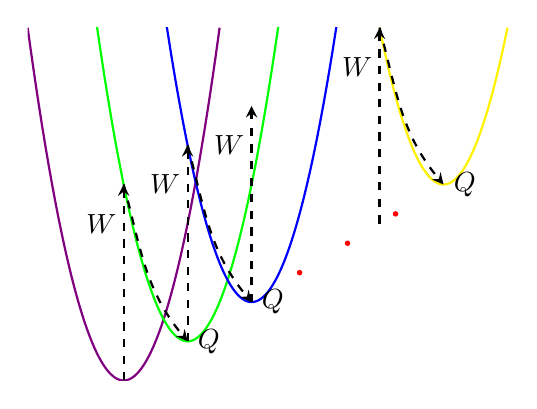
\begin{tikzpicture}
	\def\lims{xmin=-3,xmax=14,ymin=-0.001,ymax=9}
	\begin{axis}[\lims,hide x axis, hide y axis,width=0.7\textwidth,height=0.5\textwidth]
	\addplot[thick,violet,mark=none,samples=1000,domain=-3:3,y domain=-0.001:9] {0+(x-0)*(x-0)};
	\addplot[thick,green,mark=none,samples=1000,domain=-1:5,y domain=-0.001:9] {1+(x-2)*(x-2)};
	\addplot[thick,blue,mark=none,samples=1000,domain=1:7,y domain=-0.001:9] {2+(x-4)*(x-4)};
	\fill[red] (axis cs:5.5,2.75) circle[radius=1pt];
	\fill[red] (axis cs:7,3.5) circle[radius=1pt];
	\fill[red] (axis cs:8.5,4.25) circle[radius=1pt];
	\addplot[thick,yellow,mark=none,samples=1000,domain=8:12,y domain=-0.001:9] {5+(x-10)*(x-10)};
	\draw[thick,dashed,->,>=stealth] (axis cs:0,0) to (axis cs:0,5);
	\draw[thick,dashed,->,>=stealth] (axis cs:2,1) to (axis cs:2,6);
	\draw[thick,dashed,->,>=stealth] (axis cs:4,2) to (axis cs:4,7);
	\draw[thick,dashed,->,>=stealth] (axis cs:8,4) to (axis cs:8,9);
	\draw (axis cs:0-0.7,4) node{$W$};
	\draw (axis cs:2-0.7,5) node{$W$};
	\draw (axis cs:4-0.7,6) node{$W$};
	\draw (axis cs:8-0.7,8) node{$W$};
	\draw[thick,dashed,->,>=stealth] (axis cs:0,5) to [out=285,in=130] (axis cs:2,1) node[right]{$Q$};
	\draw[thick,dashed,->,>=stealth] (axis cs:2,6) to [out=285,in=130] (axis cs:4,2) node[right]{$Q$};
	\draw[thick,dashed,->,>=stealth] (axis cs:8,9) to [out=285,in=130] (axis cs:10,5) node[right]{$Q$};
	
	\end{axis}
	
	\end{tikzpicture}
	\caption{The accumulation of work and heat along a nonequilibrium trajectory. The work is defined as the energy change when the coupling parameter switches from $\lambda_i$ to $\lambda_{i+1}$ with the coordinates fixed, while the dissipated heat is defined as the energy relaxation when the coordinate change with the coupling parameter fixed.}\label{Fig:FEM:NEW}
\end{figure}

%\begin{figure}[htbp]
%	\centering
%	\includegraphics[width=0.4\textwidth]{figures/NEW.pdf}\\
%	\caption{The accumulation of work and heat along a nonequilibrium trajectory. The work is defined as the energy change when the coupling parameter switches from $\lambda_i$ to $\lambda_{i+1}$ with the coordinates fixed, while the dissipated heat is defined as the energy relaxation when the coordinate change with the coupling parameter fixed.}\label{Fig:FEM:NEW}
%\end{figure}

In Ref.~\cite{CrooksJSP1998}, Crooks showed that the distributions of work values from the forward and the backward paths satisfy a relation that is central to the histogram methods in free energy calculations
\begin{equation}
    \frac{p_{f}[w=W(\tau)]}{p_{b}[w=-\underline{W}(\tau)]}=\exp[\beta(w-\Delta A)],
    \label{Eq:FEM:NEW:crooks}
\end{equation}
where $p_{f}[w=W(\tau)]$ and $p_{b}[w=-\underline{W}(\tau)]$ are the probability densities of the work values in the forward and the reverse transformations (with a sign change for the work in the reverse path). Both are normalized, i.e., $\int p_{f}(w) \diff w=\int p_{b}(w) \diff w=1$. It is noted that Jarzynski equality Eq.~\ref{Eq:FEM:NEW:Jar} follows from Eq.~\ref{Eq:FEM:NEW:crooks} simply by integration over $w$ because the probability densities are normalized to 1:
\begin{equation}
    \int p_{f}(w)e^{-\beta w}\diff w=\int p_{b}(w)e^{-\beta \Delta A}\diff w,
    \label{Eq:FEM:NEW:crookstojar}
\end{equation}
Because of the normalization condition, the right-hand side is equal to $\exp(-\beta \Delta A)$, and Jarzynski equality follows. The bias, variance and mean square error of the Jarzynski estimator were studied by Gore et al.\cite{GorePNAS2003}

Following the Crooks Fluctuation Theorem (CFT),\cite{CrooksJSP1998} Bennett acceptance ratio can be applicable to nonequilibrium calculations. This approach was combined with a maximum likelihood estimate, and accurate free energy differences were obtained.\cite{ShirtsPRL2003}
In this approach, $\Delta A$ is calculated via
\begin{align}
    \sum_{i=1}^{n_{F}}\frac{1}{1+\exp \left[\beta(M+W_{i}-\Delta A)\right]} = \sum_{j=1}^{n_{R}}\frac{1}{1+\exp \left[-\beta(M+W_{j}-\Delta A)\right]},
    \label{Eq:FEM:NEW:NEBAR}
\end{align}
where $n_{F}$ and $n_{R}$ are the numbers of the forward and reverse transformations respectively, $W_{i}$ and $W_{j}$ are the work of forward and reverse measurements respectively, and $M=\beta^{-1}\ln(n_{F}/n_{R})$.
The corresponding statistical variance of $ \Delta A $, $ \sigma^2 $, is calculated using Eq.~10 in Ref.~\cite{ShirtsPRL2003}.

\subsubsection{Non-Equilibrium Work for Free Energy Profiles\label{Sec:FEM:NEW:FEP}}
When calculating the free energy profile in a pulling experiment, the Jarzynski equality is no longer straightforwardly applicable, because it relates the nonequilibrium work to free energy differences at different times, not positions along a predefined reaction coordinate. In order to surmount this difficulty, Hummer and Szabo extended the Jarzynski equality by measuring force/extension along pulling.\cite{HummerPNAS2001}

Let us begin with a system of which the phase-space density evolves according to a Liouville-type equation:
\begin{equation}
	\frac{\partial f(\mathbf{x},t)}{\partial t}=\mathscr{L}_tf(\mathbf{x},t).
	\label{Eq:FEM:NEW:Liouville}
\end{equation}
$\mathscr{L}_t$ is an explicitly time-dependent evolution operator that has the Boltzmann distribution as a stationary solution, $\mathscr{L}_t e^{-\beta \mathscr{H}(\mathbf{x},t)}=0$, where $\mathscr{H}(\mathbf{x},t)$ is a time-dependent Hamiltonian. For diffusive dynamics on a potential $V(\mathbf{x},t)$, the time evolution is governed by $\mathscr{L}_t=D\nabla e^{-\beta V(\mathbf{x},t)}\nabla e^{\beta V(\mathbf{x},t)}$, where $D$ is the diffusion coefficient and $\nabla=\partial/\partial \mathbf{x}$. Now consider the unnormalized Boltzmann distribution at time $t$,
\begin{align}
	p(\mathbf{x},t)=\frac{e^{-\beta \mathscr{H}(\mathbf{x},t)}}{\displaystyle\int e^{-\beta \mathscr{H}(\mathbf{x}^\prime,0)} \diff\mathbf{x}^\prime}.
\end{align}
Because this distribution is stationary ($\mathscr{L}_tp=0$), and because $\partial p/\partial t=-\beta(\partial \mathscr{H}/\partial t)p$, it follows that the above $p(\mathbf{x},t)$ is a solution of the sink equation
\begin{align}
	\frac{\partial p}{\partial t}=\mathscr{L}_tp-\beta\frac{\partial \mathscr{H}}{\partial t}p,
\end{align}
of which the solution, starting from an equilibrium distribution at time $t=0$, can be expressed as a path integral by using the Feynman-Kac theorem. Equating these two differential solutions immediately gives:
\begin{equation}
	\frac{e^{-\beta\mathscr{H}(\mathbf{x},t)}}{\displaystyle\int e^{-\beta \mathscr{H}(\mathbf{x}^\prime,0)} \diff \mathbf{x}^\prime}=\left\langle \delta(\mathbf{x}-\mathbf{x}_t)\exp{\left[-\beta\int_0^t\frac{\partial \mathscr{H}}{\partial t^\prime}(\mathbf{x}_{t^{\prime}},t^{\prime})\diff t^\prime\right]}\right\rangle.
	\label{Eq:FEM:NEW:SinkFK}
\end{equation}
The average $\left\langle \cdots \right\rangle$ is over an ensemble of trajectories starting from the equilibrium distribution at $t=0$ and evolving according to Eq.~\ref{Eq:FEM:NEW:Liouville}. Each trajectory is weighted with the Boltzmann factor of the external work $w_t$ done to the system,
\begin{equation}
	w_t=\int_0^t\frac{\partial \mathscr{H}}{\partial t^\prime}(\mathbf{x}_{t^{\prime}},t^{\prime})\diff t^\prime.
\end{equation}
Integrating on both sides of Eq.~\ref{Eq:FEM:NEW:SinkFK} with respect to $\mathbf{x}$, we obtain Jarzynski equality
\begin{equation}
	e^{-\beta \Delta G(t)}\equiv \frac{\displaystyle\int e^{-\beta\mathscr{H}(\mathbf{x},t)}\diff \mathbf{x}}{\displaystyle\int e^{-\beta \mathscr{H}(\mathbf{x},0)} \diff \mathbf{x}}=\left \langle e^{-\beta w_t}\right\rangle
\end{equation}
between the Boltzmann-averaged work $w_t$ and the equilibrium free energy difference $\Delta G(t)$ between times $t$ and $0$.

In a single-molecule pulling experiment, e.g. using atomic force microscope (AFM), the sample is moved at a constant speed $v$ relative to the cantilever with spring constant $k$. The position $z_t=vt+\delta z_t$ of the cantilever tip with respect to the sample is recorded, where $\delta z_t$ is the displacement of the cantilever tip. It can be described by a Hamiltonian $\mathscr{H}(\mathbf{x},t)=\mathscr{H}_0(\mathbf{x})+k(z(\mathbf{x})-vt)^2/2$, where $\mathscr{H}_0(\mathbf{x})$ is the Hamiltonian of the resting, unperturbed system. \textit{It is worth noting that $\mathscr{H}(\mathbf{x},t)$ is the Hamiltonian for the total system, including the cantilever.} Substituting this Hamiltonian into Eq.~\ref{Eq:FEM:NEW:SinkFK}, multiplying both sides by $\delta[z-z(\mathbf{x})]$, and integrating over all $\mathbf{x}$, we have
\begin{align}
	\frac{\displaystyle\int\delta[z-z(\mathbf{x})]e^{-\beta \left\{\mathscr{H}_0(\mathbf{x})+k[z(\mathbf{x})-vt]^2/2\right\}}\diff \mathbf{x}}{\displaystyle\int e^{-\beta \mathscr{H}(\mathbf{x},0)}\diff \mathbf{x}}=\qquad\qquad\qquad\qquad\qquad&\notag\\
	\int \delta[z-z(\mathbf{x})] \left\langle \delta(\mathbf{x}-\mathbf{x}_t)e^{-\beta\int_0^t -kv\left[z(\mathbf{x}_{t^\prime}-vt^\prime)\right] \diff t^\prime}\right\rangle \diff \mathbf{x}\notag\\
	\frac{\displaystyle\int\delta[z-z(\mathbf{x})]e^{-\beta \mathscr{H}_0(\mathbf{x})}\diff \mathbf{x}}{\displaystyle\int e^{-\beta \mathscr{H}(\mathbf{x},0)}\diff \mathbf{x}}e^{-\beta k(z-vt)^2/2}=\qquad\qquad\qquad\qquad\qquad\quad&\notag\\
	\left\langle \delta[z-z(\mathbf{x_{t}})] e^{-\beta \left[-kv\int_0^t z(\mathbf{x}_{t^\prime})\diff t^\prime+kv^2t^2/2\right]}\right\rangle\notag\\
	\frac{\displaystyle\int\delta[z-z(\mathbf{x})]e^{-\beta \mathscr{H}_0(\mathbf{x})}\diff \mathbf{x}}{\displaystyle\int e^{-\beta \mathscr{H}(\mathbf{x},0)}\diff \mathbf{x}}=\qquad\qquad\qquad\qquad\qquad\qquad\qquad\qquad&\notag\\
	\left\langle \delta[z-z(\mathbf{x_{t}})] e^{-\beta \left[kv^2t^2/2-kv\int_0^t z(\mathbf{x}_{t^\prime})\diff t^\prime-k(z(\mathbf{x}_t)-vt)^2/2\right]}\right\rangle
\end{align}
and finally taking the logarithm, we have:
\begin{align}
	G_0(z)\equiv&-\beta^{-1}\ln{\frac{\displaystyle\int\delta[z-z(\mathbf{x})]e^{-\beta \mathscr{H}_0(\mathbf{x})}\diff \mathbf{x}}{\displaystyle\int e^{-\beta \mathscr{H}_0(\mathbf{x})}\diff \mathbf{x}}}\notag\\
	      =&-\beta^{-1}\ln{\left<\delta(z-z_t)e^{-\beta \Delta w_t}\right>}-\beta^{-1}\ln{\frac{\displaystyle\int e^{-\beta \mathscr{H}_0(\mathbf{x})+k[z(\mathbf{x})]^2/2}\diff \mathbf{x}}{\displaystyle\int e^{-\beta \mathscr{H}_0(\mathbf{x})}\diff \mathbf{x}}}\notag\\
	      =&-\beta^{-1}\ln{\left<\delta(z-z_t)e^{-\beta \Delta w_t}\right>}+\delta G,
\end{align}
where $G_0(z)$ is the unperturbed free energy profile along the pulling coordinate $z$, and $\Delta w_t$ is the external work minus the instantaneous biasing potential, $\Delta w_t=w_t-k(z_t-vt)^2/2=kv(vt^2/2-\int_0^t z_{t^\prime}\diff t^\prime)-k(z_t-vt)^2/2$. %The expression can be obtained by integrating the power over time. At any moment $t^\prime$, the force acting on the system is $f=k(vt^\prime-z_{t^\prime})$. Correspondingly, the power $p=f\cdot v$. Therefore, $w_t=\int p\diff t^\prime=\int_0^t kv(vt^\prime-z_{t^\prime})\diff t^\prime=kv(vt^2/2-\int_0^t z_{t^\prime}\diff t^\prime)$. 
$\delta G$ is independent of time.
At time $t=0$, the trajectories are started from points $z_0$ drawn from a Boltzmann distribution corresponding to Hamiltonian $\mathscr{H}(\mathbf{x},0)=\mathscr{H}_0(\mathbf{x})+kz^2/2$, which is \emph{NOT} $\mathscr{H}_0(\mathbf{x})$.

At each time slice $t$, one can in principle obtain an estimate of the whole free energy surface. In practice with finite number of trajectories, at any given time $t$, only a narrow region around the equilibrium position $z=vt$ will be sampled adequately. Thus, an average over several time slices and repeated trajectories is required to obtain an optimal estimate of the free energy profile. At every time slice $t$, one obtains an ensemble of positions $z_t$ and corresponding $w_t$s. The position $z_t$ are binned, and the corresponding histogram values are incremented by $e^{-\beta w_t}$. The complete free energy profile $G_0(z)$ can be reconstructed by adapting the weighted histogram method:
\begin{align}
	G_0(z)=-\beta^{-1}\ln{\frac{\sum_t \frac{\left<\delta(z-z_t)\exp{(-\beta w_t)}\right>}{\left<\exp{(-\beta w_t)}\right>}}{\sum_t\frac{\exp{[-\beta u(z,t)]}}{\left<\exp{(-\beta w_t)}\right>}}},
	\label{Eq:FEM:NEW:FEprofile}
\end{align}
where the sum is over time slices $t$ and $u(z,t)=k(z-vt)^2/2$ is the time dependent biasing potential. As in the weighted histogram method, this procedure can be refined by making Eq.~\ref{Eq:FEM:NEW:FEprofile} self-consistent through replacement of $\left<\exp{(-\beta w_t)}\right>$ with
\begin{equation}
	\exp{[-\beta \Delta G(t)]}=\frac{\displaystyle\int \exp{\left\{-\beta \left[u(z,t)+G_0(z)\right]\right\}}\diff z}{\displaystyle\int \exp{\left\{-\beta[u(z,0)+G_0(z)]\right\}\diff z}},
\end{equation}
thus requiring an iterative solution for $\Delta G(t)$. Note that Eq.~\ref{Eq:FEM:NEW:FEprofile} can be rewritten as
\begin{equation}
	G_0(z)=-\beta^{-1}\ln{\frac{\sum_t \frac{\left<\delta(z-z_t)\exp{(-\beta \Delta w_t)}\right>\exp{[-\beta u(z,t)]}}{\left<\exp{(-\beta w_t)}\right>}}{\sum_t\frac{\exp{[-\beta u(z,t)]}}{\left<\exp{(-\beta w_t)}\right>}}},
\end{equation}
which is the natural logarithm of the weighted average of $\left<\delta(z-z_t)\exp{(-\beta \Delta w_t)}\right>$ over all the time slices with $\frac{\exp{[-\beta u(z,t)]}}{\left<\exp{(-\beta w_t)}\right>}$ being the weight.
\clearpage 
\input {chapters/TRAM.tex}
\clearpage 
\section{Approximate Methods}
\input {chapters/MMPBSA.tex}